\documentclass[12pt]{article}

\title{Application of Machine Learning Coursework Report}
\author{James Hughes \\ Word Count: 2904}

\usepackage{graphicx}
\usepackage{subcaption}
\usepackage[export]{adjustbox}
\usepackage{multirow}
\usepackage[hidelinks]{hyperref}
\usepackage{url}
\def\UrlBreaks{\do\/\do-}

\begin{document}

\maketitle

\newpage

\tableofcontents

\newpage

\section{Gaussian Noise Diffusion}
\subsection{Diffusion Model \& Training Algorithm}
The code found in the repository for this project was based on the Jupyter notebook found in the \texttt{assignment} directory.
This notebook contains a standard pipeline which trains a Denoising Diffusion Probabilistic Model,
a kind of generative model first appearing in the literature just four years ago \cite{ho2020denoising}.
The model is trained using the training partition of the MNIST dataset \cite{mnist}, which contains monochrome images of handwritten digits.

Fundamental to this model is an underlying image-to-image convolutional neural network,
which tries to predict a ground truth MNIST image from the same image, with added Gaussian noise, as an input.
This network has a deep, symmetrical architecture based on convolutional layers which initially increase the number of channels,
which extracts features from the input, and then later combines these channels to eventually produce a monochrome (single-channel) generated image.
These convolutional layers are combined with a layer normalisation,
which normalises the pre-activations of the hidden units separately for each input of the batch \cite{ba2016layer}.
This technique builds on the earlier batch normalisation approach, improving the stability and speed of training the neural network \cite{ba2016layer},
but has the advantage of being more suitable when batches are small or have a large within-batch variation \cite{prince2023understanding}.
The results of the layer normalisation are then passed through a GeLU activation function \cite{hendrycks2023gaussian},
which is a close variant of the standard ReLU activation function,
but which mitigates the issue of vanshing gradients by having non-zero gradients for small negative inputs \cite{nguyen2021analysis}.

The underlying CNN model also takes a scalar time step \texttt{t} in $[0,1]$ as part of its raw input; this becomes a vector when inputs are batched,
with one scalar for each batch member.
Each of these scalars is in turn encoded as a vector, whose entries are a periodic function (of progressively increasing frequency)
of the scalar value.
These vectors are then passed through a series of learned linear layers and non-linear activations,
changing their length to equal the number of hidden channels in the first layer of the CNN.
These time embeddings are then combined with the first hidden activations via addition.

This underlying model is then wrapped in a \texttt{DDPM} class, implementing a \texttt{forward} and \texttt{sample} method.
The \texttt{forward} method takes a batch of MNIST images as input.
It generates a random time step for each image, which controls the strength of degradation applied to each,
taking the form of addition with Gaussian pixel noise.
It feeds the degraded image and the time step to the CNN, and returns the mean squared error between the CNN output and the original noise map.
During training this encourages the CNN to predict the Gaussian noise applied to a degraded image.
The \texttt{sample} method implements Algorithm 18.2 in \cite{prince2023understanding}.
It starts with a random Gaussian tensor the same size as the MNIST images, which it then passes through the trained CNN,
and subsequently degrades with Gaussian noise.
These two transformations are repeated for smaller and smaller timesteps until the degradation is minimal, and a synthetic image is generated.

The initial codebase was created by refactoring this notebook into a package, \texttt{diffusiontools}.
The training procedure was then altered to make training runs more repeatable.
Alongside the samples which were produced at each epoch, the trained model was itself saved as a \texttt{.pt} file.
This enabled further investigation into intermediate models after the training, and indeed meant that later on,
the periodic sampling could be removed altogether to speed up training (as sampling could be done afterwards).
The hyperparameter settings were also controlled via a \texttt{config.ini} file to enable different configurations to be easily tested, and tracked.

\subsection{Analysis of Training}

\begin{figure}[hp]
    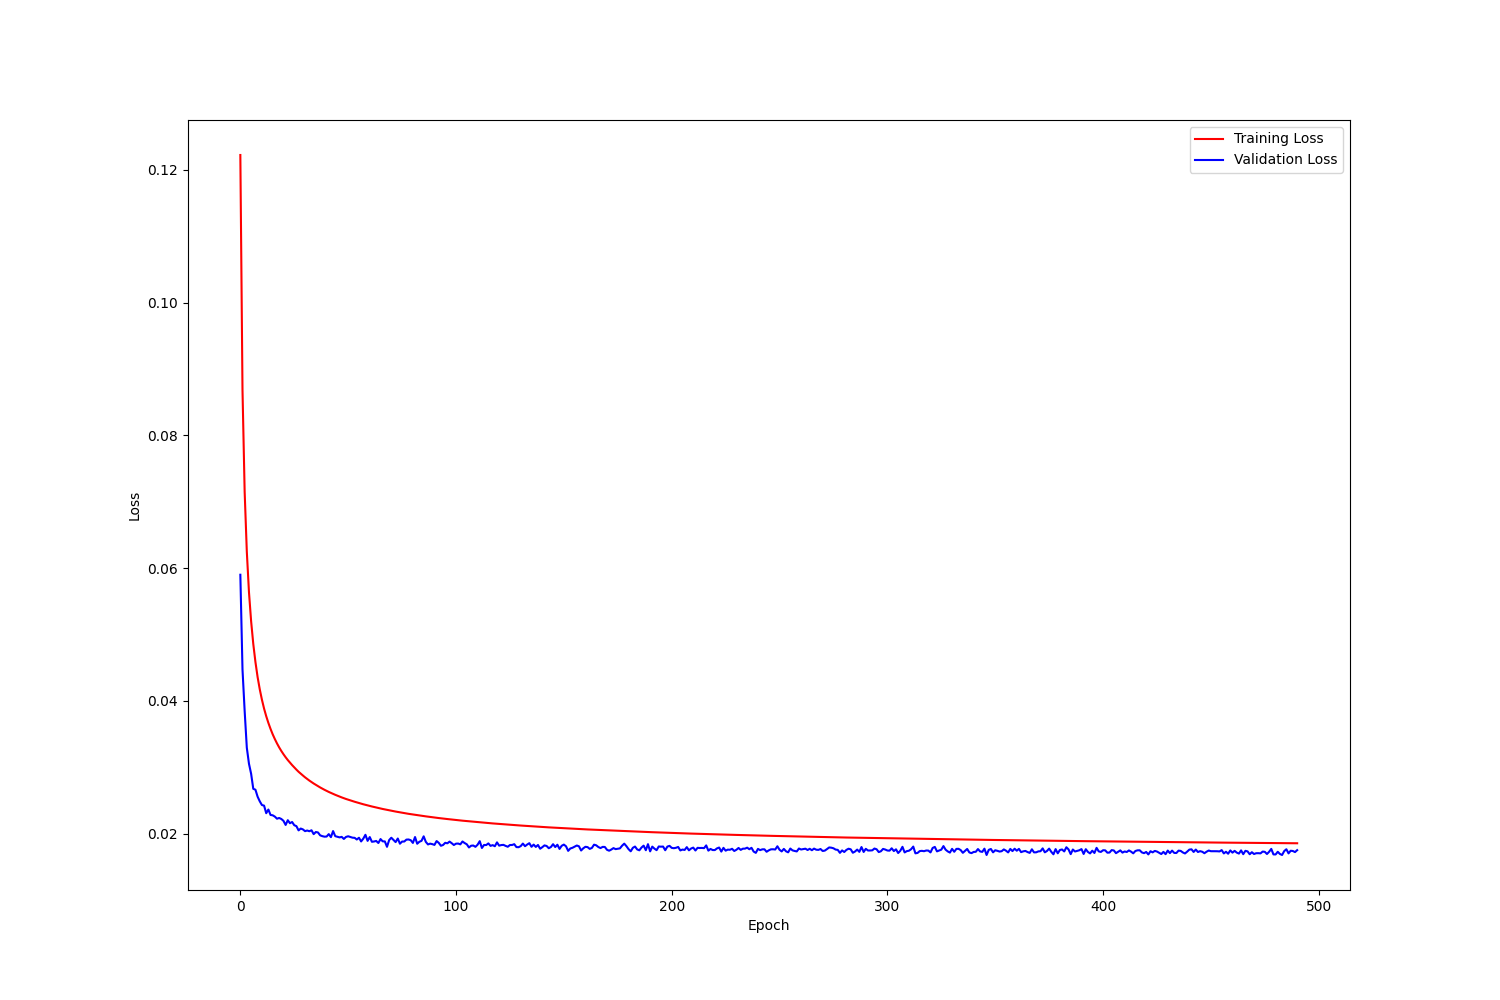
\includegraphics[scale=0.35, center]{figures/learning_curve_1.png}
    \caption{Learning Curve for Model 1 Trained over 500 Epochs.}
    \label{fig:learning_curve_1}
\end{figure}

The first model trained had the same hyperparameters as found in the notebook.
It was trained for 500 epochs by uploading the repository to the CSD3 systems.
The MNIST training dataset was split further into a training set (80\%) and a validation set (20\%),
to monitor the model's ability to generalise during the training process.

In Figure \ref{fig:learning_curve_1}, it can be seen that the validation loss appears to converge roughly around the 100 epoch stage,
with no significant improvements from further training.
This matches the findings of generated samples in Figure \ref{fig:diffusion_1}.
We see that around the 40 epoch mark, the model begins to produce symbols but these are not recognisable digits.
The images generated at epoch 60 are the first that resemble numerical digits --
images in Figure \ref{fig:diffusion_1}\ref{sub@fig:1_60} appear to show a 7, 5, 2, 1, and 9.
Figure \ref{fig:diffusion_1}\ref{sub@fig:1_120} appears to show higher fidelity images in the first three samples,
although the other two cannot be discerned as digits.
This model was selected for further analysis as the final trained model.

\begin{figure}[hp]
    \begin{subfigure}{0.49\textwidth}
    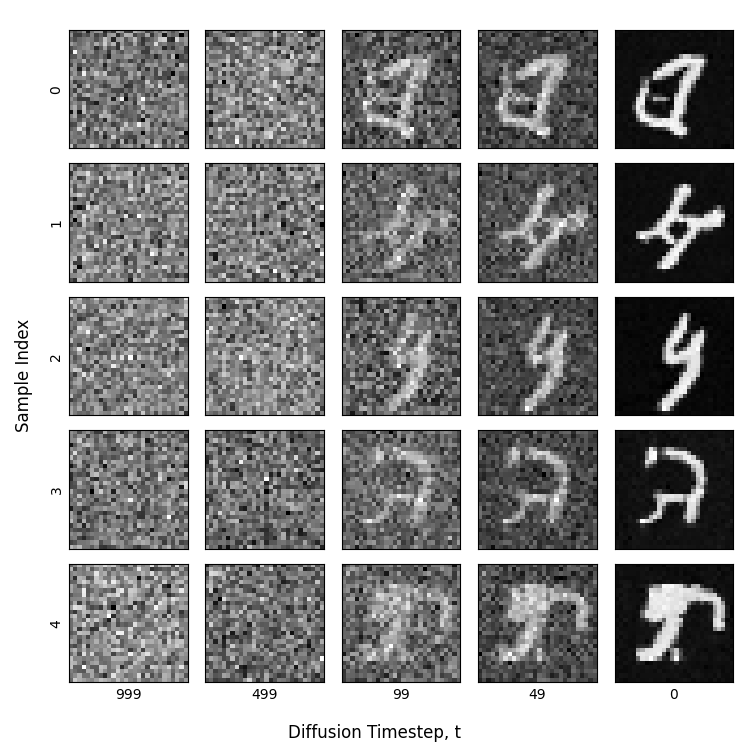
\includegraphics[width=0.9\linewidth, height=6cm, center]{figures/diffusion_plot_1_0040.png}
    \caption{Epoch 40}
    \label{fig:1_40}
    \end{subfigure}
    \begin{subfigure}{0.49\textwidth}
    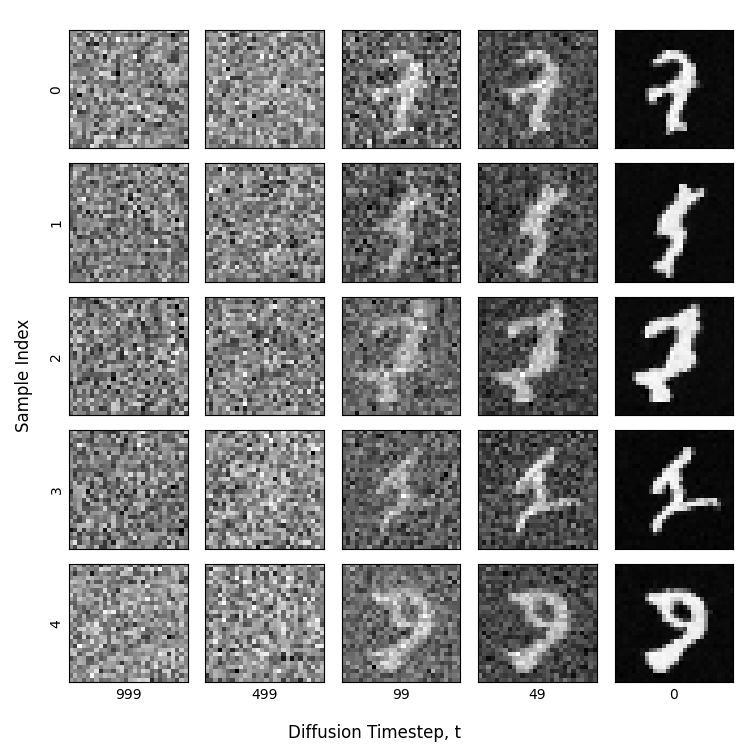
\includegraphics[width=0.9\linewidth, height=6cm, center]{figures/diffusion_plot_1_0060.png}
    \caption{Epoch 60}
    \label{fig:1_60}
    \end{subfigure}

    \begin{subfigure}{0.49\textwidth}
    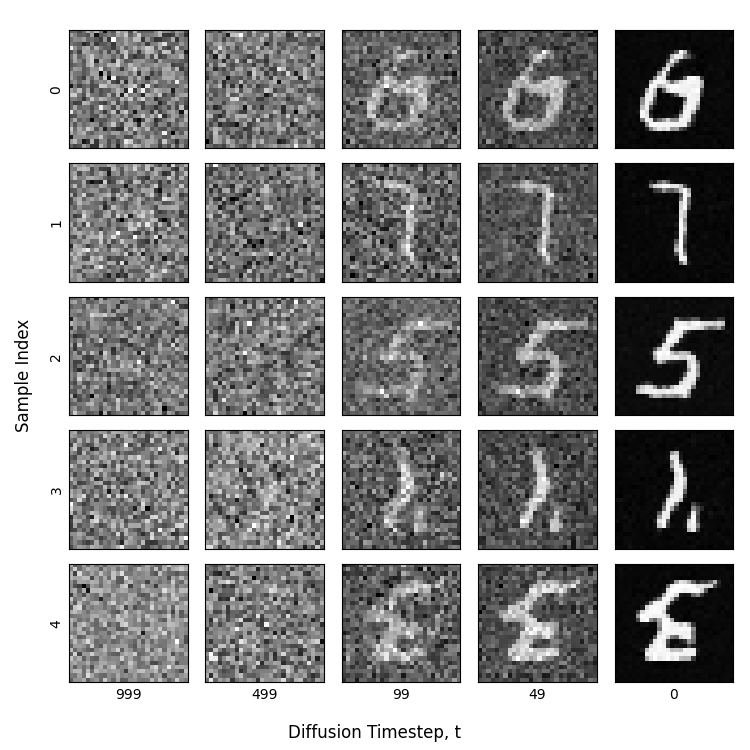
\includegraphics[width=0.9\linewidth, height=6cm, center]{figures/diffusion_plot_1_0120.png}
    \caption{Epoch 120}
    \label{fig:1_120}
    \end{subfigure}
    \begin{subfigure}{0.49\textwidth}
    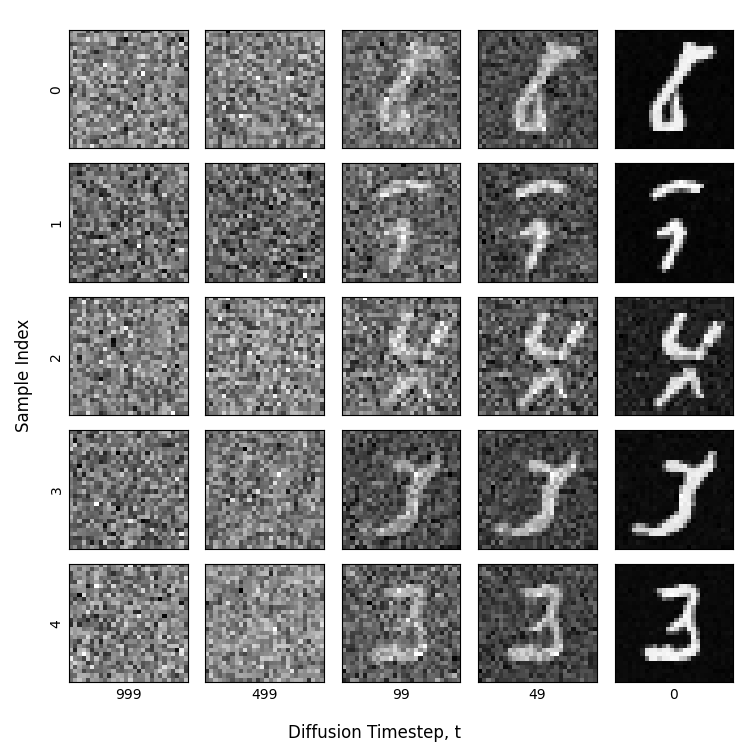
\includegraphics[width=0.9\linewidth, height=6cm, center]{figures/diffusion_plot_1_0300.png}
    \caption{Epoch 300}
    \label{fig:1_300}
    \end{subfigure}

    \caption{Model 1 diffusion process samples at various stages of training.}
    \label{fig:diffusion_1}
\end{figure}

A second similar model was then trained with a slightly different Gaussian noising schedule.
In this second model, the number of discrete timesteps in the diffusion process was reduced ten-fold to 100.
The noise parameter limits were accordingly increased by a factor of ten, ensuring that the amount of signal-to-noise ratio of an image at the final time step remained approximately zero.


\begin{figure}[hp]
    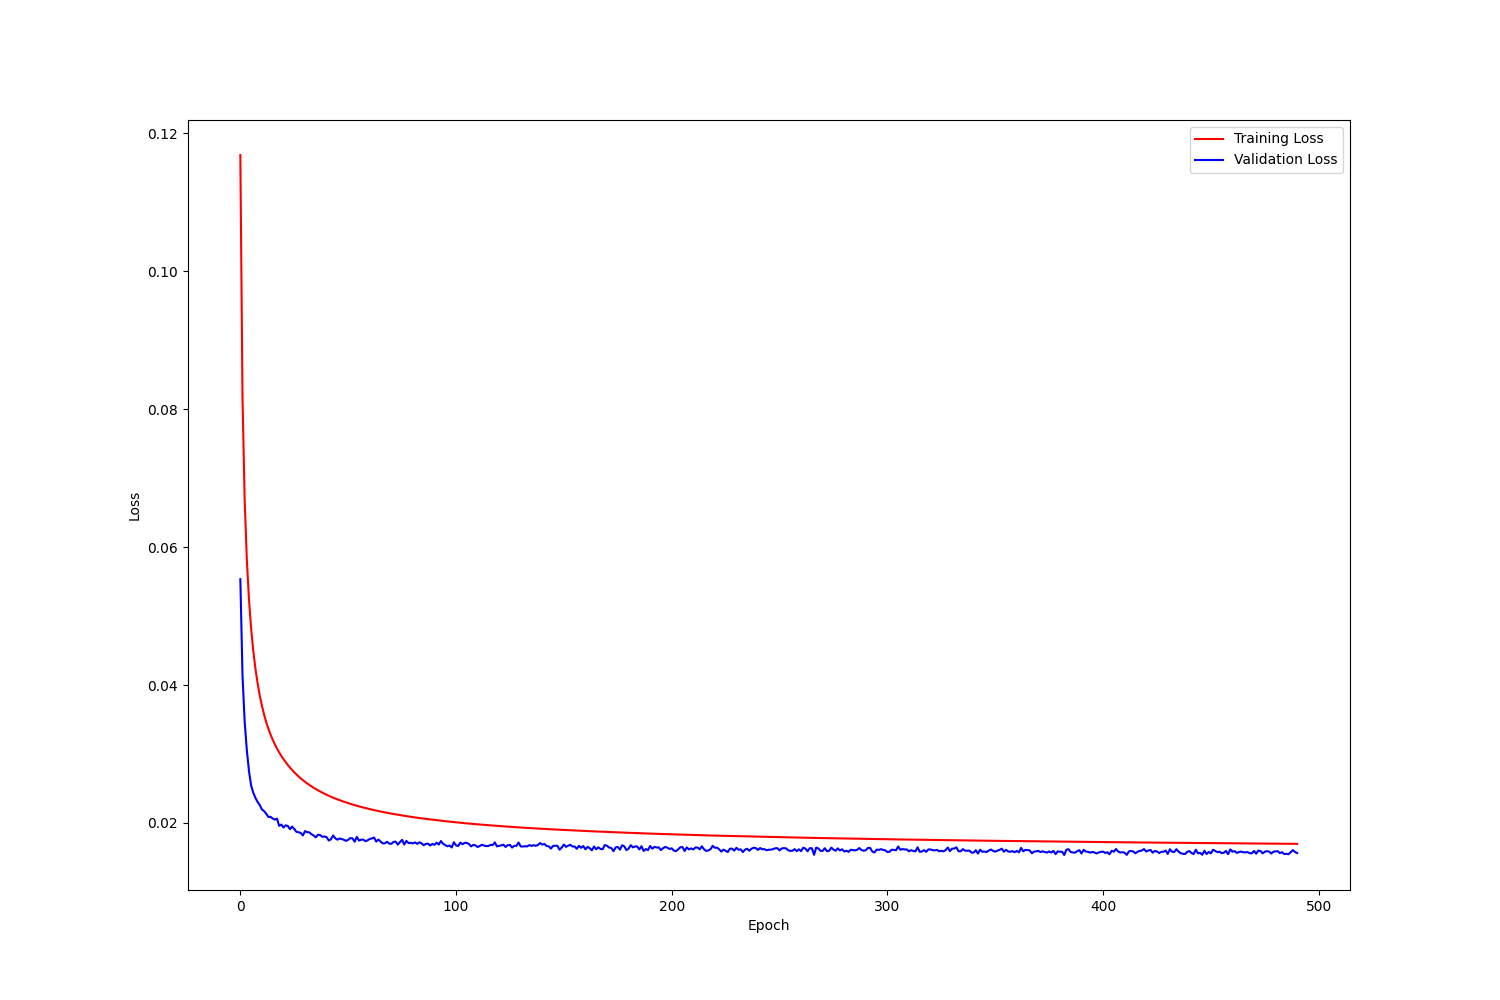
\includegraphics[scale=0.35, center]{figures/learning_curve_2.png}
    \caption{Learning Curve for Model 2 Trained over 500 Epochs.}
    \label{fig:learning_curve_2}
\end{figure}

\begin{figure}[hp]
    \begin{subfigure}{0.49\textwidth}
    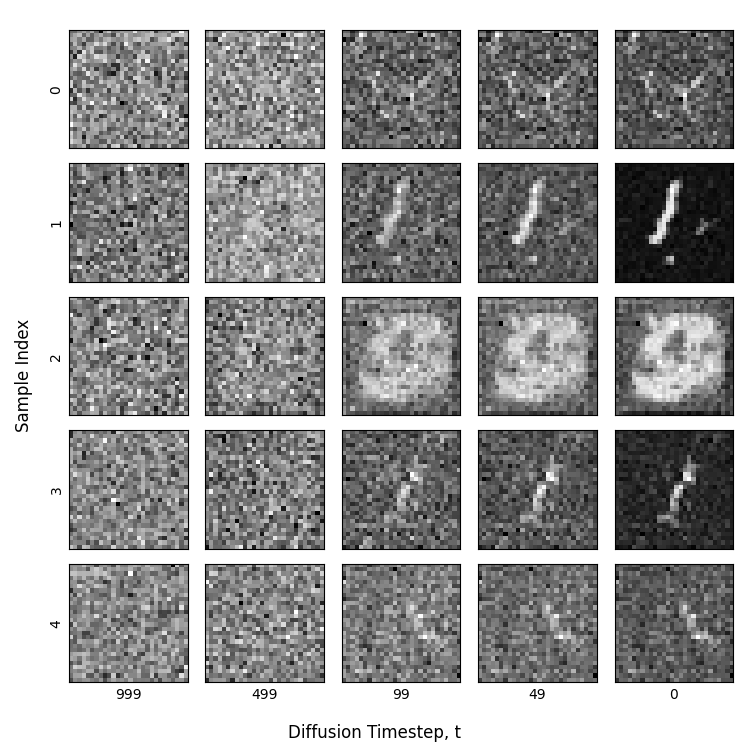
\includegraphics[width=0.9\linewidth, height=6cm, center]{figures/diffusion_plot_2_0020.png}
    \caption{Epoch 20}
    \label{fig:2_20}
    \end{subfigure}
    \begin{subfigure}{0.49\textwidth}
    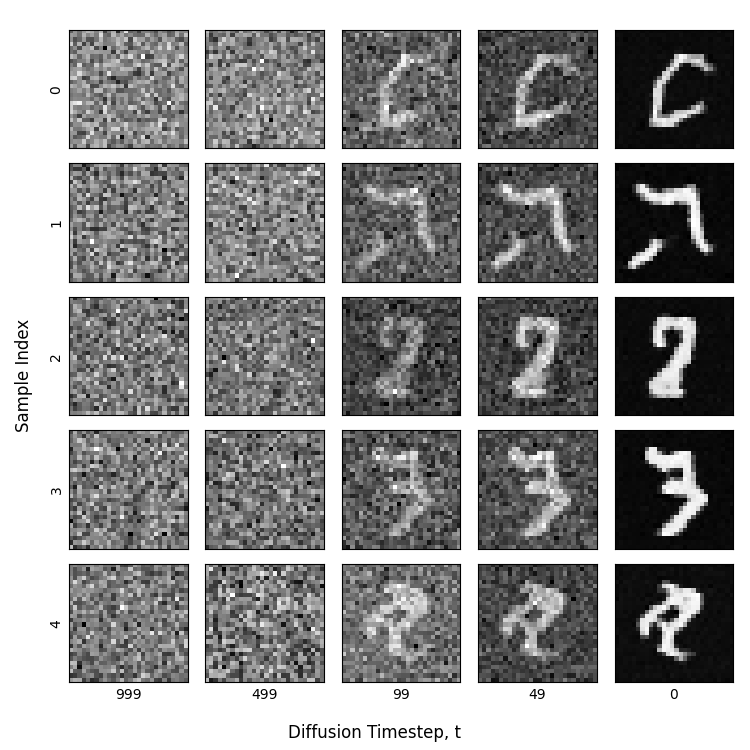
\includegraphics[width=0.9\linewidth, height=6cm, center]{figures/diffusion_plot_2_0040.png}
    \caption{Epoch 40}
    \label{fig:2_40}
    \end{subfigure}

    \begin{subfigure}{0.49\textwidth}
    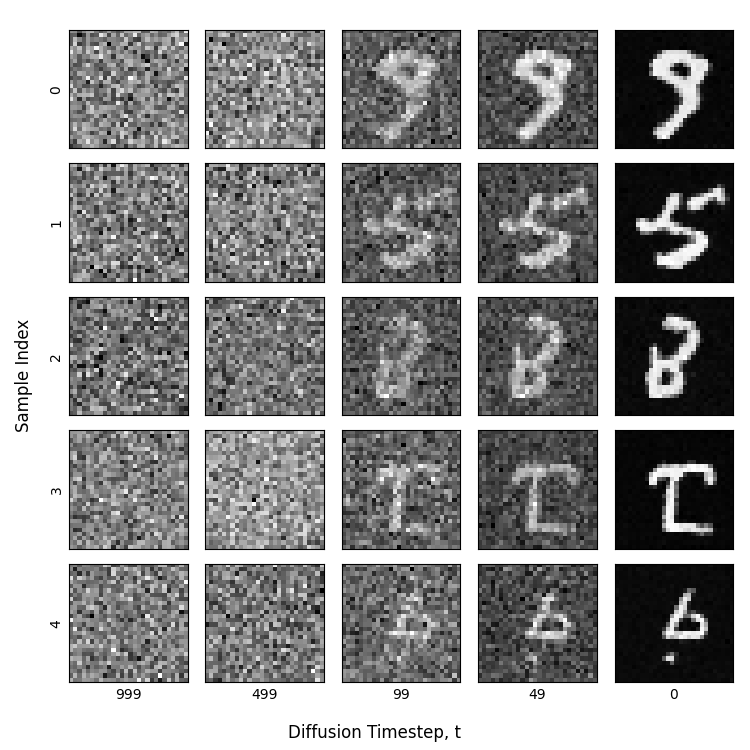
\includegraphics[width=0.9\linewidth, height=6cm, center]{figures/diffusion_plot_2_0080.png}
    \caption{Epoch 80}
    \label{fig:2_80}
    \end{subfigure}
    \begin{subfigure}{0.49\textwidth}
    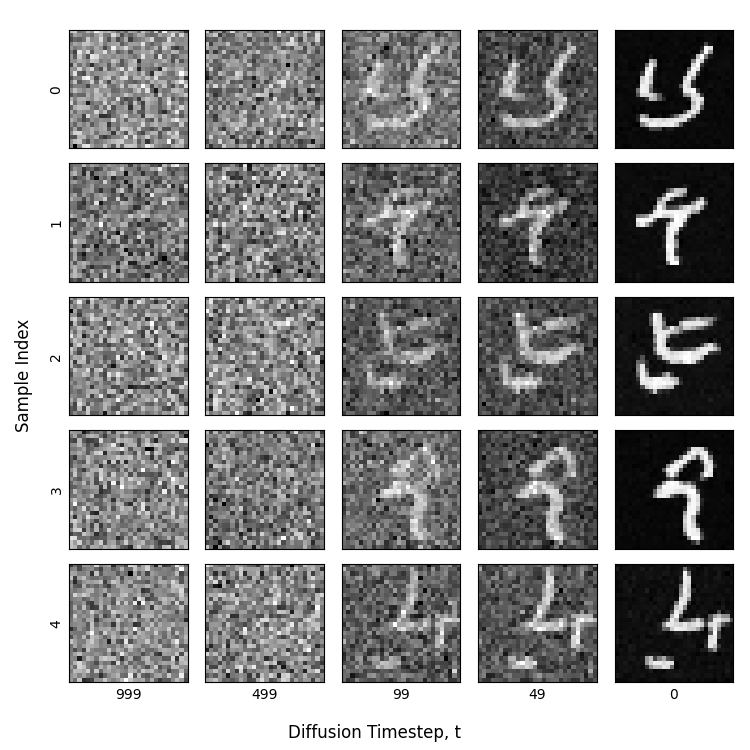
\includegraphics[width=0.9\linewidth, height=6cm, center]{figures/diffusion_plot_2_0100.png}
    \caption{Epoch 100}
    \label{fig:2_100}
    \end{subfigure}

    \caption{Model 2 diffusion process samples at various stages of training.}
    \label{fig:diffusion_2}
\end{figure}

A similar learning curve can be seen for the training of the second model in Figure \ref{fig:learning_curve_2}.
However, inspecting some of the images produced by intermediate models shows that the quality of the generated images deteriorates much earlier than in Model 1.
Even images produced at epoch 100 in Figure \ref{fig:diffusion_2} appear to be low quality, with `fragmented' symbols rather than one continuous digit.
The images produced at epoch 80 appear to be the highest quality and this model was used in the final analysis.

\subsection{Analysis of Final Models}
The evaluation of generative models is a challenging and ongoing subject of research \cite{betzalel2022study},\cite{fi15080260}.
Unlike other tasks within machine learning such as classification, regression, and clustering,
an ideal generative model generalises from its training data to produce content that is simultaneously novel, diverse and realistic.
When diffusion models are used in a conditional generation setting, ground truth images can be degraded and then reconstructed by the diffusion model,
allowing evaluation through image comparison metrics such as SSIM and MSE, as done in \cite{bansal2022cold} -- this is explored later.
More broadly, a standard evaluation metric is the Fr\'echet Inception Distance \cite{NIPS2017_8a1d6947}.
In this project, the models are quantitatively assessed with the framework of comparing the statistical distributions of generated and ground truth images,
just like with the FID score, but in a slightly simpler and more interpretable way.
200 samples were taken from each of the four final models and combined with the 10,000 MNIST test images into a single array.
These were then transformed into two dimensions using t-SNE dimensionality reduction.
The effect of this on the MNIST dataset alone can be seen in Figure \ref{fig:tsne_mnist},
which shows that this technique is strikingly effective at encoding the true image class in a meaningful way.
A Gaussian mixture model with 10 components (corresponding to the 10 digits) was then fitted to each sample,
enabling an estimate of the KL divergence between the generated and ground truth image distributions.



\begin{figure}[hp]
    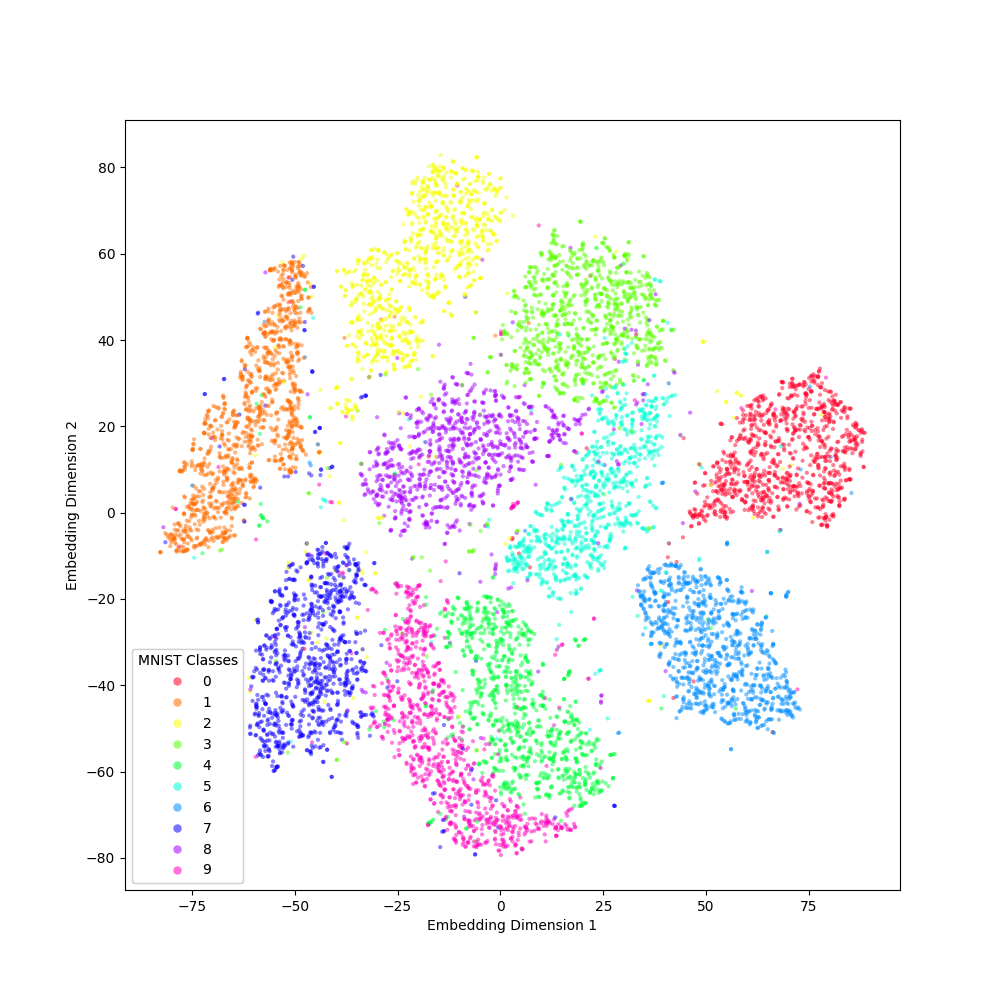
\includegraphics[scale=0.54, center]{figures/tsne_mnist.png}
    \caption{t-SNE dimensionality reduction applied to MNIST test dataset, with ground truth labels indicated.}
    \label{fig:tsne_mnist}
\end{figure}

\begin{figure}[hp]
    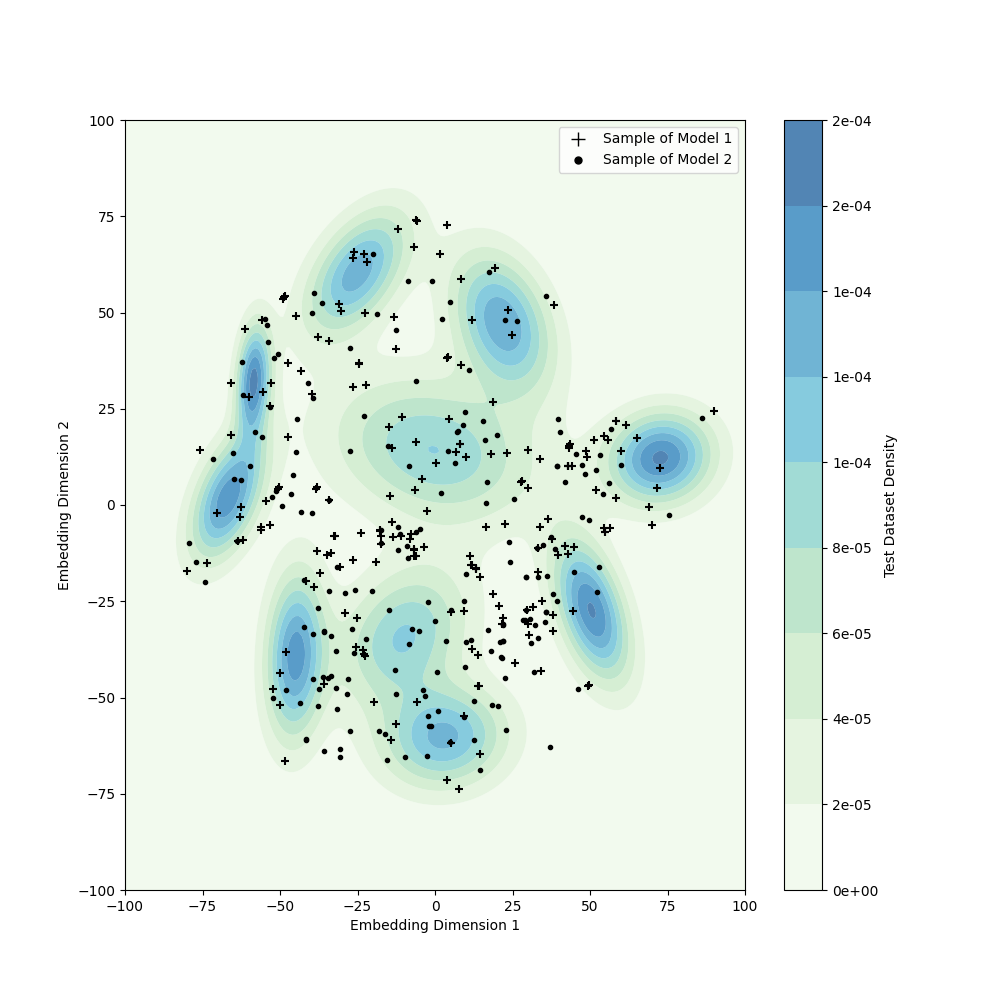
\includegraphics[scale=0.54, center]{figures/tsne_gaussian_models.png}
    \caption{t-SNE dimensionality reduction applied to Gaussian model samples, with contour plot of GMM density estimate for MNIST test data.}
    \label{fig:tsne_gaussian}
\end{figure}

Figure \ref{fig:tsne_gaussian} shows that both models have good coverage across the whole distribution of ground truth distribution of data,
suggesting they are capable of producing a variety of different digits.
However, we can also observe that neither distribution of points appears to have a similar clustering pattern to the ground truth data,
which suggests that both models also have a tendency to produce low quality samples that do correspond to a discernible digit.
The KL divergences, computed as $D_{KL}(P||Q)$ where $Q$ is the ground truth distribution, were similar with the model 1 sample at 0.81844,
and the model 2 sample at 0.77298.
This suggests that the distributions of generated images from both models imitate the ground truth with similar success.
When their images are treated as random vectors, the total variance (trace of the covariance matrix) for the first sample was 56.7,
and slightly higher for the second at 69.9.
While this may suggest a greater diversity of samples from the second model, it may also reflect the greater noise present at each step,
which in turn is clearly visible as the samples produced appear grainier.

\begin{figure}[hp]
    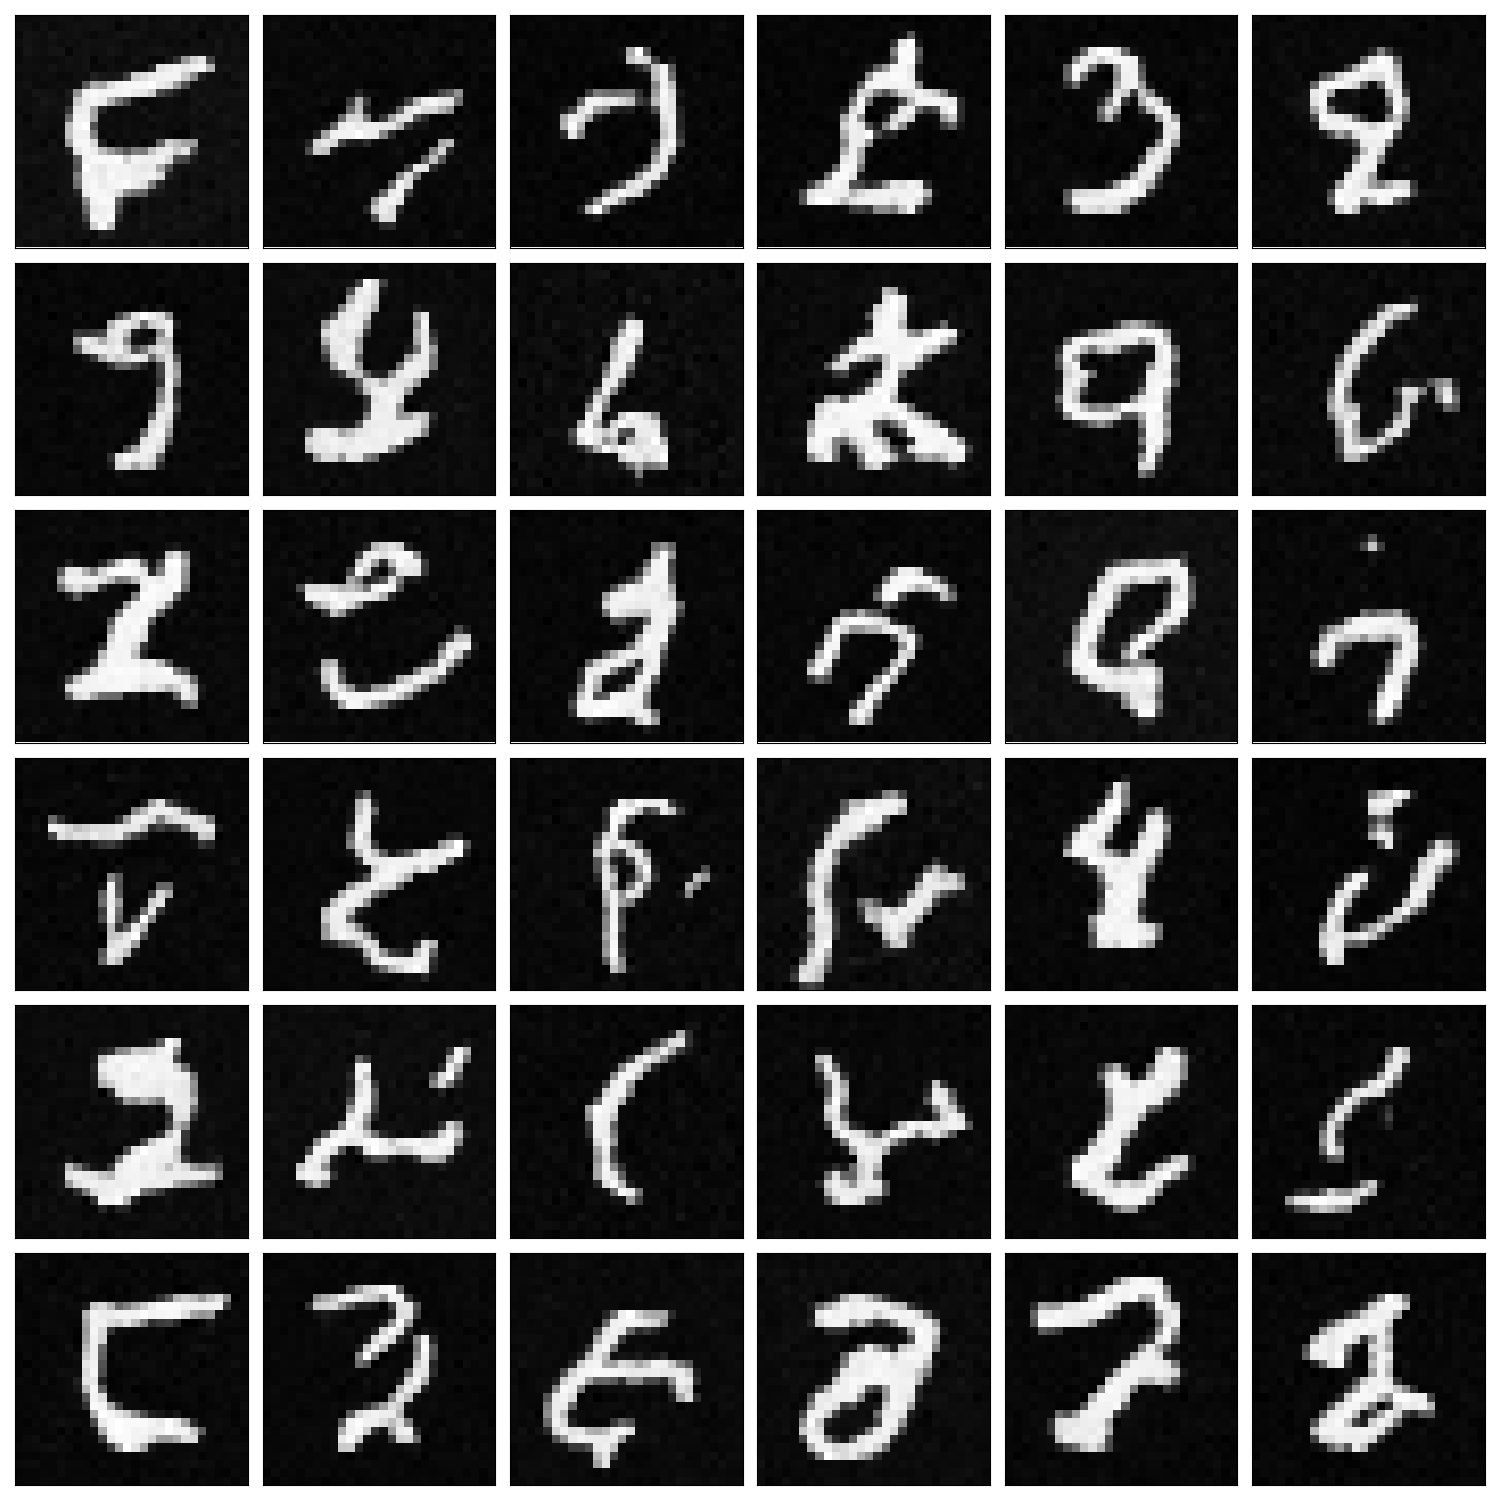
\includegraphics[scale=0.3, center]{figures/samples_1.png}
    \caption{Samples from model 1.}
    \label{fig:samples_1}
\end{figure}

\begin{figure}[hp]
    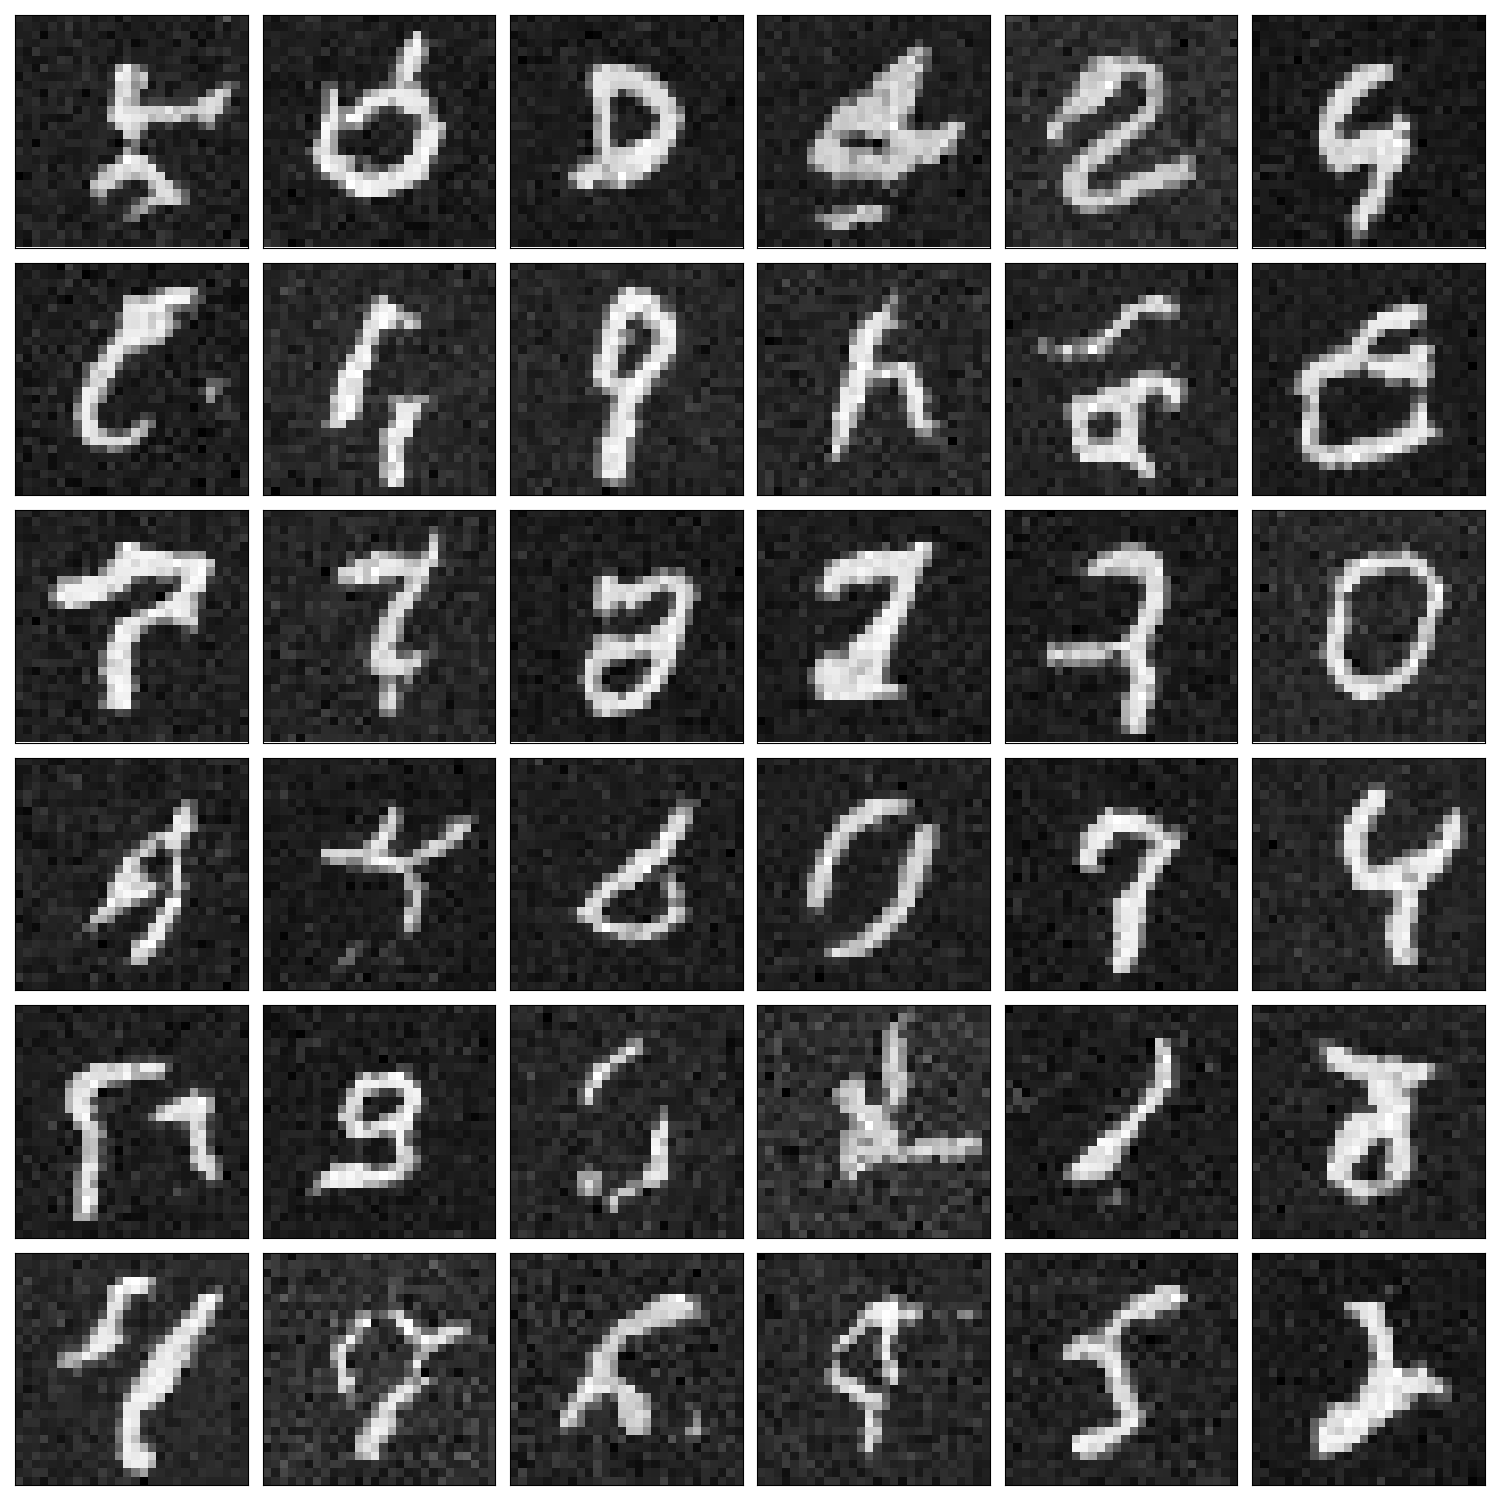
\includegraphics[scale=0.3, center]{figures/samples_2.png}
    \caption{Samples from model 2.}
    \label{fig:samples_2}
\end{figure}

\section{Custom Diffusion Model}


\subsection{Custom Degradation Strategy}

The custom degradation strategy was created to match the framework of diffusion described in \cite{bansal2022cold}.
In this paper, Bansal et al. describe a diffusion model as consisting of a degradation $D(x_0,t)$ and restoration $R(x_t, t)$ operator.
The degradation should be more severe with increasing $t$ such that there is no degradation at $t=0$,
while the restoration operator should approximate the inverse such that $R(D(x,t),t) \approx x_0$.
In our context $R$ is the learned CNN model.
For the degradation, Bansal et al. used a variety of unconventional operators.
One of the simpler examples was a super-resolution denoising model,
where the degradation was a downsampling which essentially grouped together chunks of pixels and averaged them to have a single pixel value.
This motivated the idea of grouping pixels together and permuting the groups,
so that the denoising task was somewhat akin to solving a sliding puzzle.
Here larger time steps could correspond to smaller groups of pixels so that in the extreme, all individual pixels are permuted.
However, this proved to be computationally infeasible (the degradation must be performed thousands of times for each epoch).
Instead, in the implementation, the procedure iterates through all pixels, each time swapping it with the pixel value at another random position.
This random index is chosen as the current pixel coordinates, plus a random uniform offset whose limits in both spatial directions are controlled by the noise parameter.
Therefore at small time steps pixel values are only swapped locally.
This custom degradation strategy is illustrated in Figure \ref{fig:custom}.

\begin{figure}[hp]
    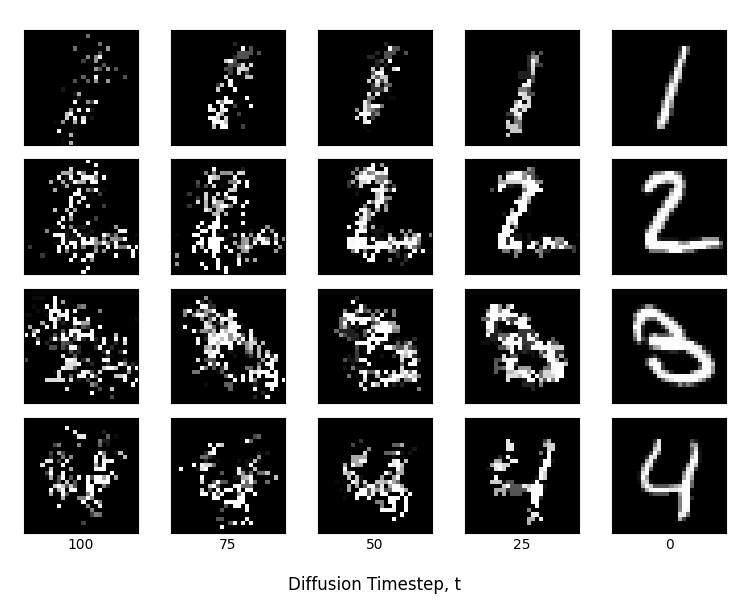
\includegraphics[scale=0.7, center]{figures/custom_degradation.png}
    \caption{Examples of the custom degradation operator with different noise levels, acting on test MNIST images.}
    \label{fig:custom}
\end{figure}

\begin{figure}[hp]
    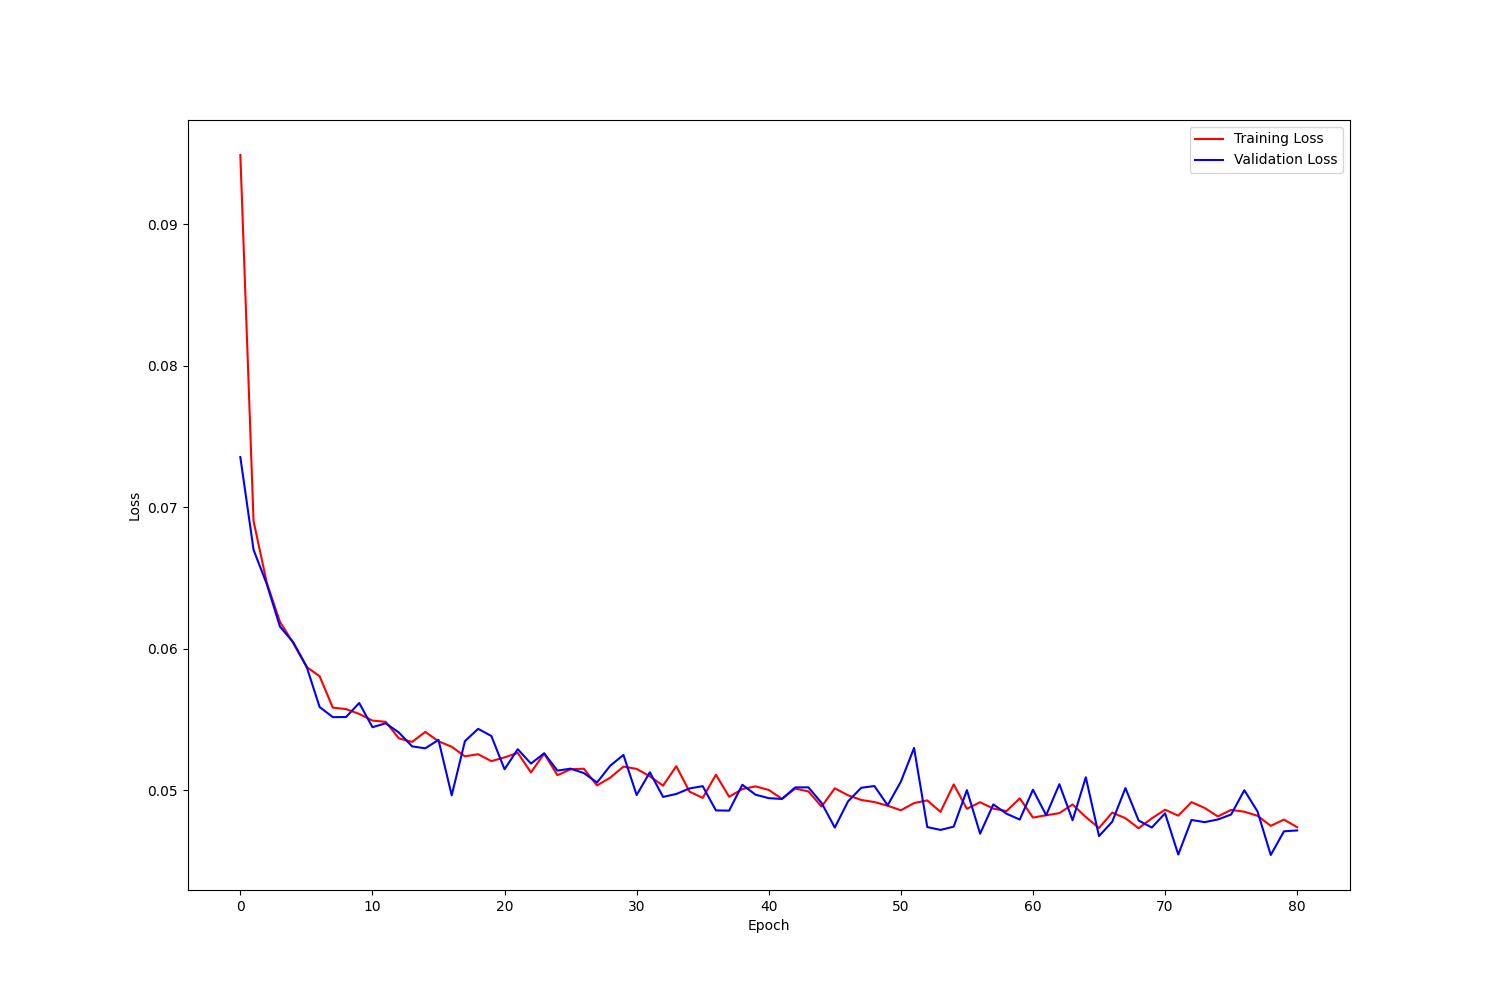
\includegraphics[scale=0.4, center]{figures/learning_curve_9.png}
    \caption{Learning curve of first custom diffusion model.}
    \label{fig:learning_curve_9}
\end{figure}


One limitation of the implementation of this model is that since the noise is not additive,
the degradation process for a single image takes a considerable amount of compute time,
which then scales with the batch size.
To mitigate this, the \texttt{forward} method of the new model class \texttt{DMCustom} applies the same degradation noise level to the whole batch,
so that the random swapping index can be computed once for each pixel,
and the corresponding pixel in all batch images can be swapped simultaneously via the tensor API.
In this way, each batch step involves the same random time step for the whole batch rather than a vector of time steps.
In turn this may mean that the training regime is less stable since there will be heterogeneity across different batches.

\subsection{Analysis of Custom Diffusion Training}

In the first instance this model was implemented with slightly different hyperparameters.
The number of time steps was set to 100, and the batch size was set to 64, in order to try to mitigate the aforementioned stability issue.
The initial learning rate was reduced to $10^{-4}$ to counteract the increased noise from the smaller batches.
Additionally an L1 loss was used, just as in \cite{bansal2022cold}.

This model was only trained for 80 epochs, which was sufficient to observe it's loss curve plateau (Figure \ref{fig:learning_curve_9}).
Moreover, we can see that the quality of trained samples reaches an optimum much earlier than this in Figure \ref{fig:diffusion_9}, around epoch 20.
Past this point, the diversity of samples falls dramatically, with almost excusively ones produced.
A possible explanation for this is that the degradation has an asymmetrical nature,
in the sense that moderate degradation is much more likely to transform a complex symbol (for instance a 6 that contains a loop) into a simple continuous `blob',
than the other way around.
This would explain the cartoonish, thick-stroked quality of the final samples produced by this model.
Another related issue is that the final time-step noise level is likely not strong enough in this sample;
this can be seen in Figure \ref{fig:custom} which uses the same noise levels, where the most noisy images can still be discerned as their true digits.

\begin{figure}[hp]
    \begin{subfigure}{0.49\textwidth}
    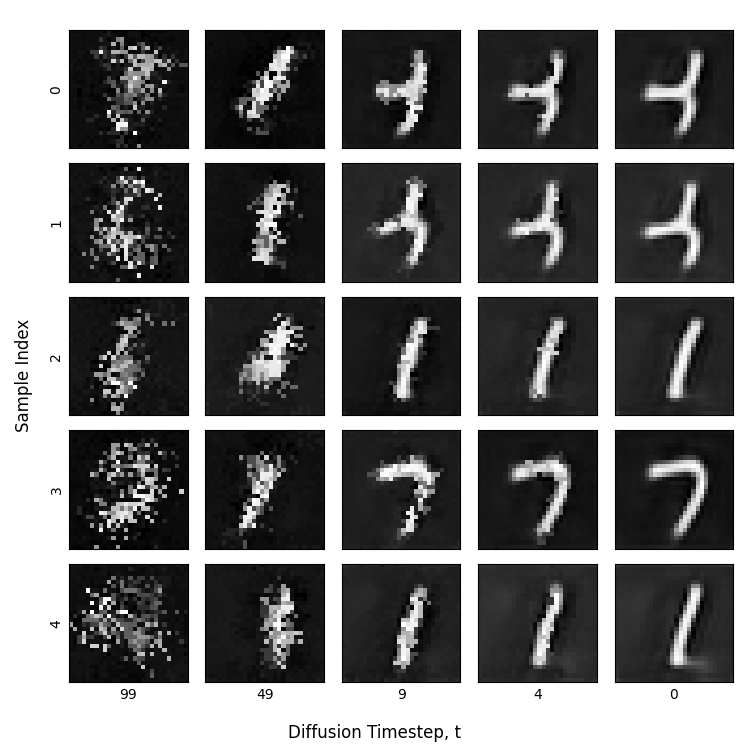
\includegraphics[width=0.9\linewidth, height=6cm, center]{figures/diffusion_plot_9_0000}
    \caption{Epoch 0}
    \label{fig:9_0}
    \end{subfigure}
    \begin{subfigure}{0.49\textwidth}
    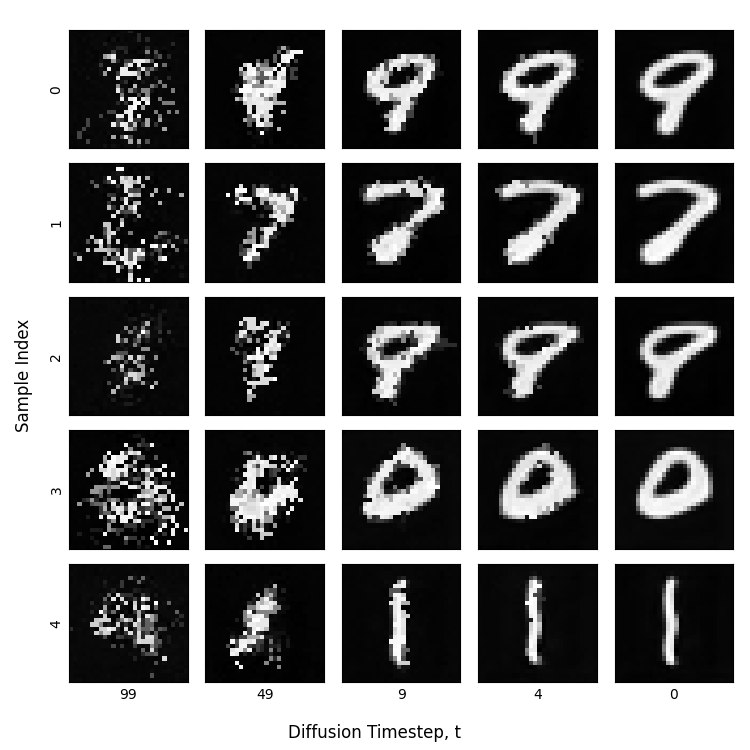
\includegraphics[width=0.9\linewidth, height=6cm, center]{figures/diffusion_plot_9_0020.png}
    \caption{Epoch 20}
    \label{fig:9_20}
    \end{subfigure}

    \begin{subfigure}{0.49\textwidth}
    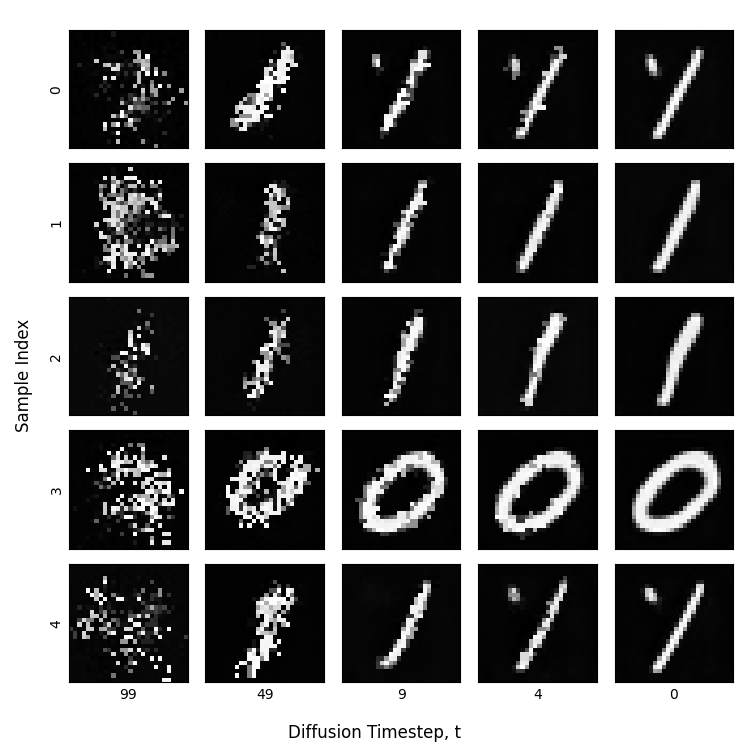
\includegraphics[width=0.9\linewidth, height=6cm, center]{figures/diffusion_plot_9_0060.png}
    \caption{Epoch 60}
    \label{fig:9_60}
    \end{subfigure}
    \begin{subfigure}{0.49\textwidth}
    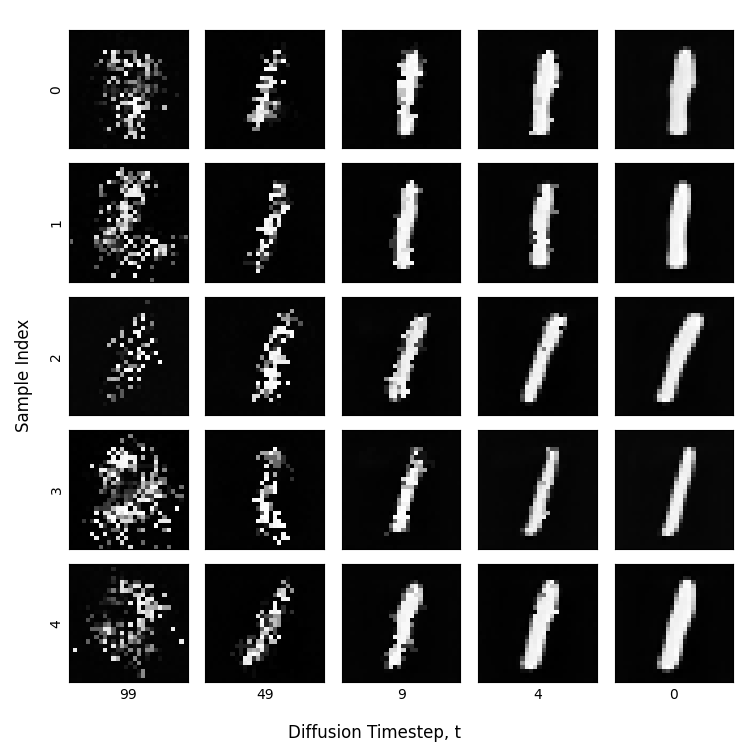
\includegraphics[width=0.9\linewidth, height=6cm, center]{figures/diffusion_plot_9_0080.png}
    \caption{Epoch 80}
    \label{fig:9_80}
    \end{subfigure}

    \caption{First custom diffusion process samples at various stages of training.}
    \label{fig:diffusion_9}
\end{figure}

In the second model, the final noise level was increased, and the total number of time steps was reduced from 100 to 20,
to reduce the accumulation of apparent bias towards 1s inherent in the degradation scheme.
The loss was changed back to L2.
This was trained for 180 epochs, although the loss appears to begin to plateau around epoch 140 in Figure \ref{fig:learning_curve_10} which is also where the best quality samples appear to be produced.
Interestingly, this model has very low sample diversity immediately from epoch 0, as seen in Figure \ref{fig:diffusion_9}
It begins to produce reasonable images of digits around epoch 40, but this is mostly 8s and 9s.
Sampels from epoch 180 seem to revert to lower levels of diversity again, and with low quality images.

\begin{figure}[hp]
    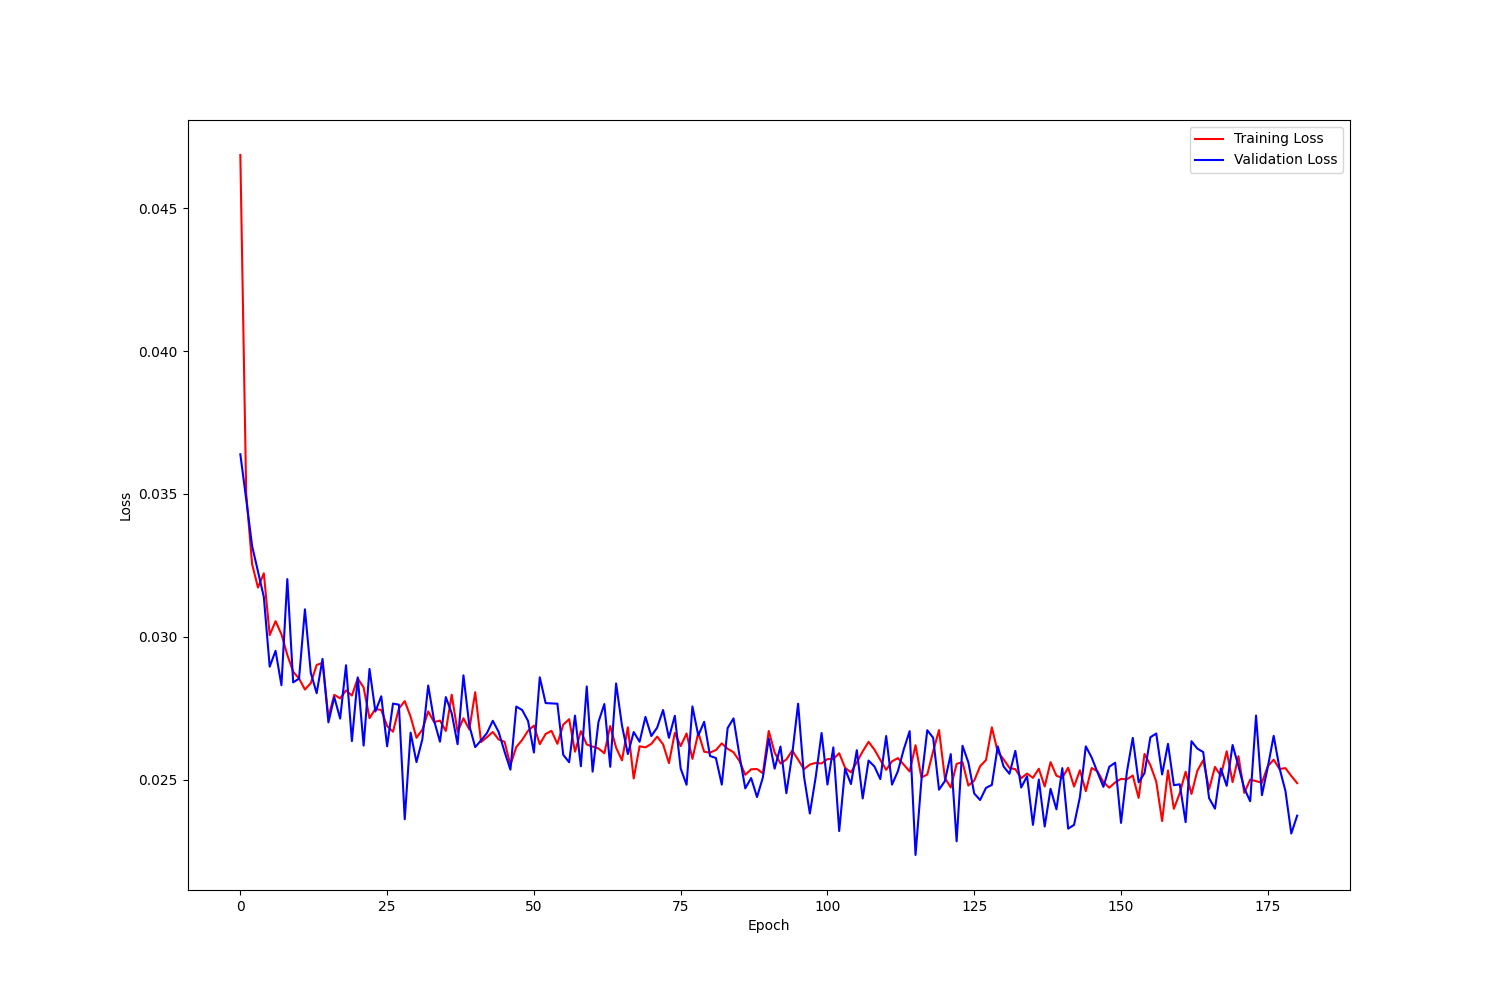
\includegraphics[scale=0.4, center]{figures/learning_curve_10.png}
    \caption{Learning curve of second custom diffusion model.}
    \label{fig:learning_curve_10}
\end{figure}

\begin{figure}[hp]
    \begin{subfigure}{0.49\textwidth}
    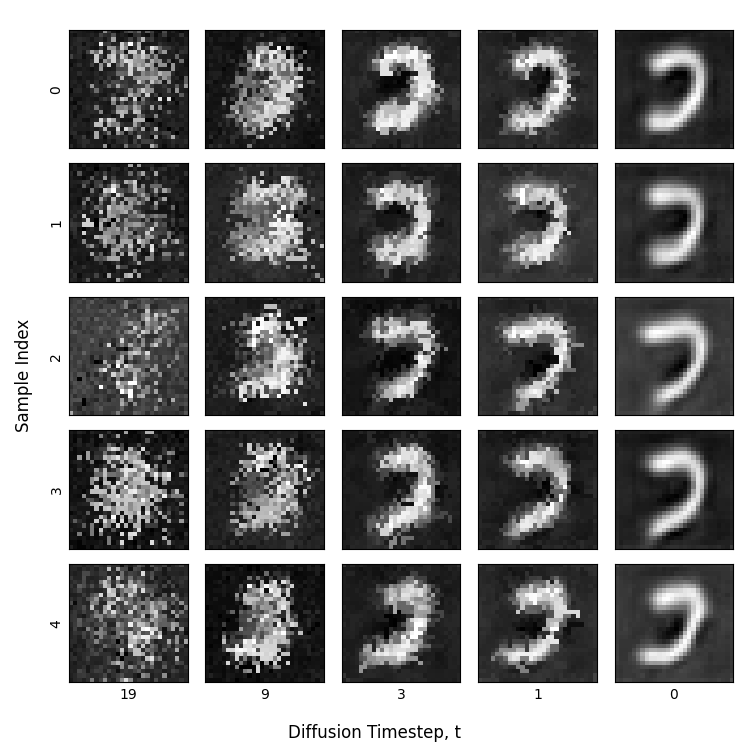
\includegraphics[width=0.9\linewidth, height=6cm, center]{figures/diffusion_plot_10_0000.png}
    \caption{Epoch 0}
    \label{fig:10_0}
    \end{subfigure}
    \begin{subfigure}{0.49\textwidth}
    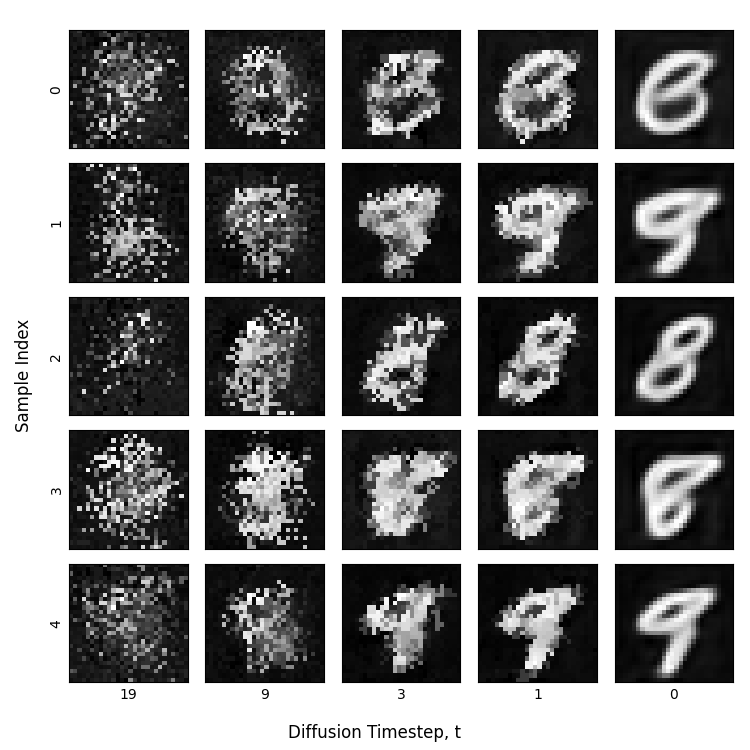
\includegraphics[width=0.9\linewidth, height=6cm, center]{figures/diffusion_plot_10_0040.png}
    \caption{Epoch 40}
    \label{fig:10_40}
    \end{subfigure}

    \begin{subfigure}{0.49\textwidth}
    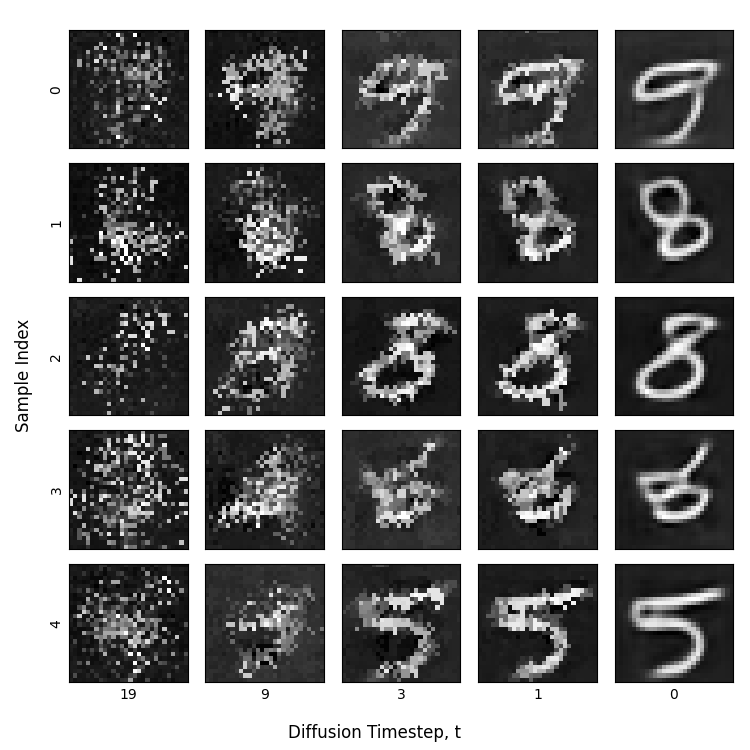
\includegraphics[width=0.9\linewidth, height=6cm, center]{figures/diffusion_plot_10_0140.png}
    \caption{Epoch 140}
    \label{fig:10_140}
    \end{subfigure}
    \begin{subfigure}{0.49\textwidth}
    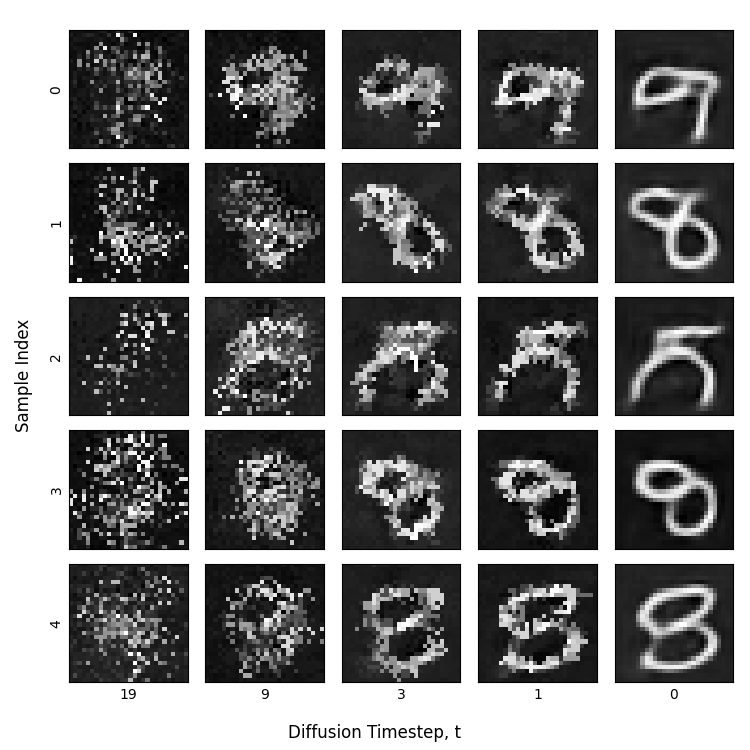
\includegraphics[width=0.9\linewidth, height=6cm, center]{figures/diffusion_plot_10_0180.png}
    \caption{Epoch 180}
    \label{fig:10_180}
    \end{subfigure}

    \caption{Second custom diffusion process samples at various stages of training.}
    \label{fig:diffusion_10}
\end{figure}

In Figure \ref{fig:tsne_custom}, we see the same t-SNE embeddings of samples of images produced from the two custom models.
Both samples appear to have multiple significant clusters of points concentrated in small areas,
which suggests that the generated samples are not particularly diverse -- this is especially evident for the first custom diffusion model.
However, the second sample does have a slightly lower total variance at 41.5, compared to 49.1 for the first model's images.

Unlike the first degradation scheme, the distribution of maximally degraded images under the custom scheme is intractable and difficult to sample from.
This is unlike the Gaussian noise scheme where the diffusion sampling begins with a random image generated from an isotropic Gaussian distribution.
In the implementation custom scheme, this initial `seed' is generated as a sample from the MNIST test data, which is maximally degraded according to the maximum noise level.
In this sense, the model can also be used in a conditional generation setting.
This is demonstrated in Figure \ref{fig:cond_generation}, which shows the original ground truth image prior to degradation,
followed by the reconstruction produced by one application of the denoising model,
and then the image generated by the standard diffusion process, similar to Figure 3 in \cite{bansal2022cold}.

\begin{figure}[hp]
    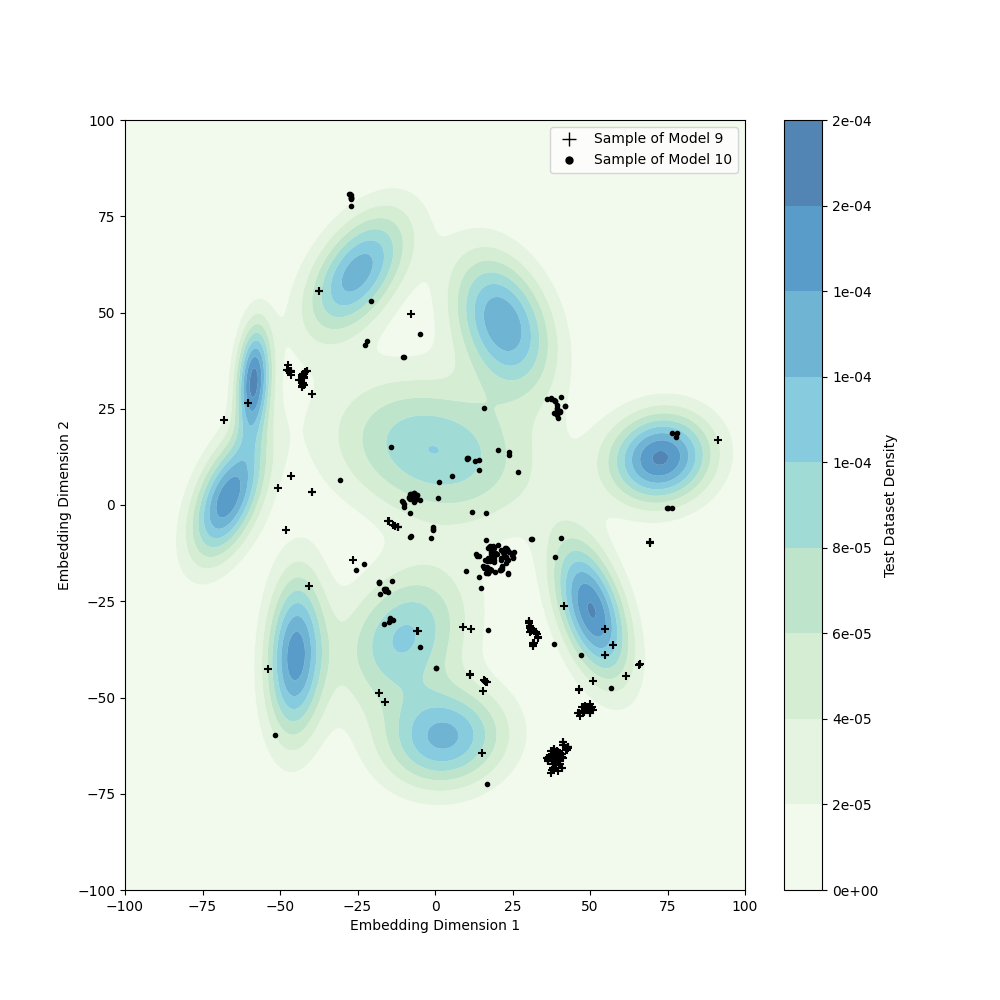
\includegraphics[scale=0.54, center]{figures/tsne_custom_models.png}
    \caption{t-SNE dimensionality reduction applied to custom model samples, with contour plot of GMM density estimate for MNIST test data. (NB: `Model 9' and `Model 10' refer to the first and second models respectively.)}
    \label{fig:tsne_custom}
\end{figure}

\begin{figure}[hp]
    \begin{subfigure}{0.49\textwidth}
    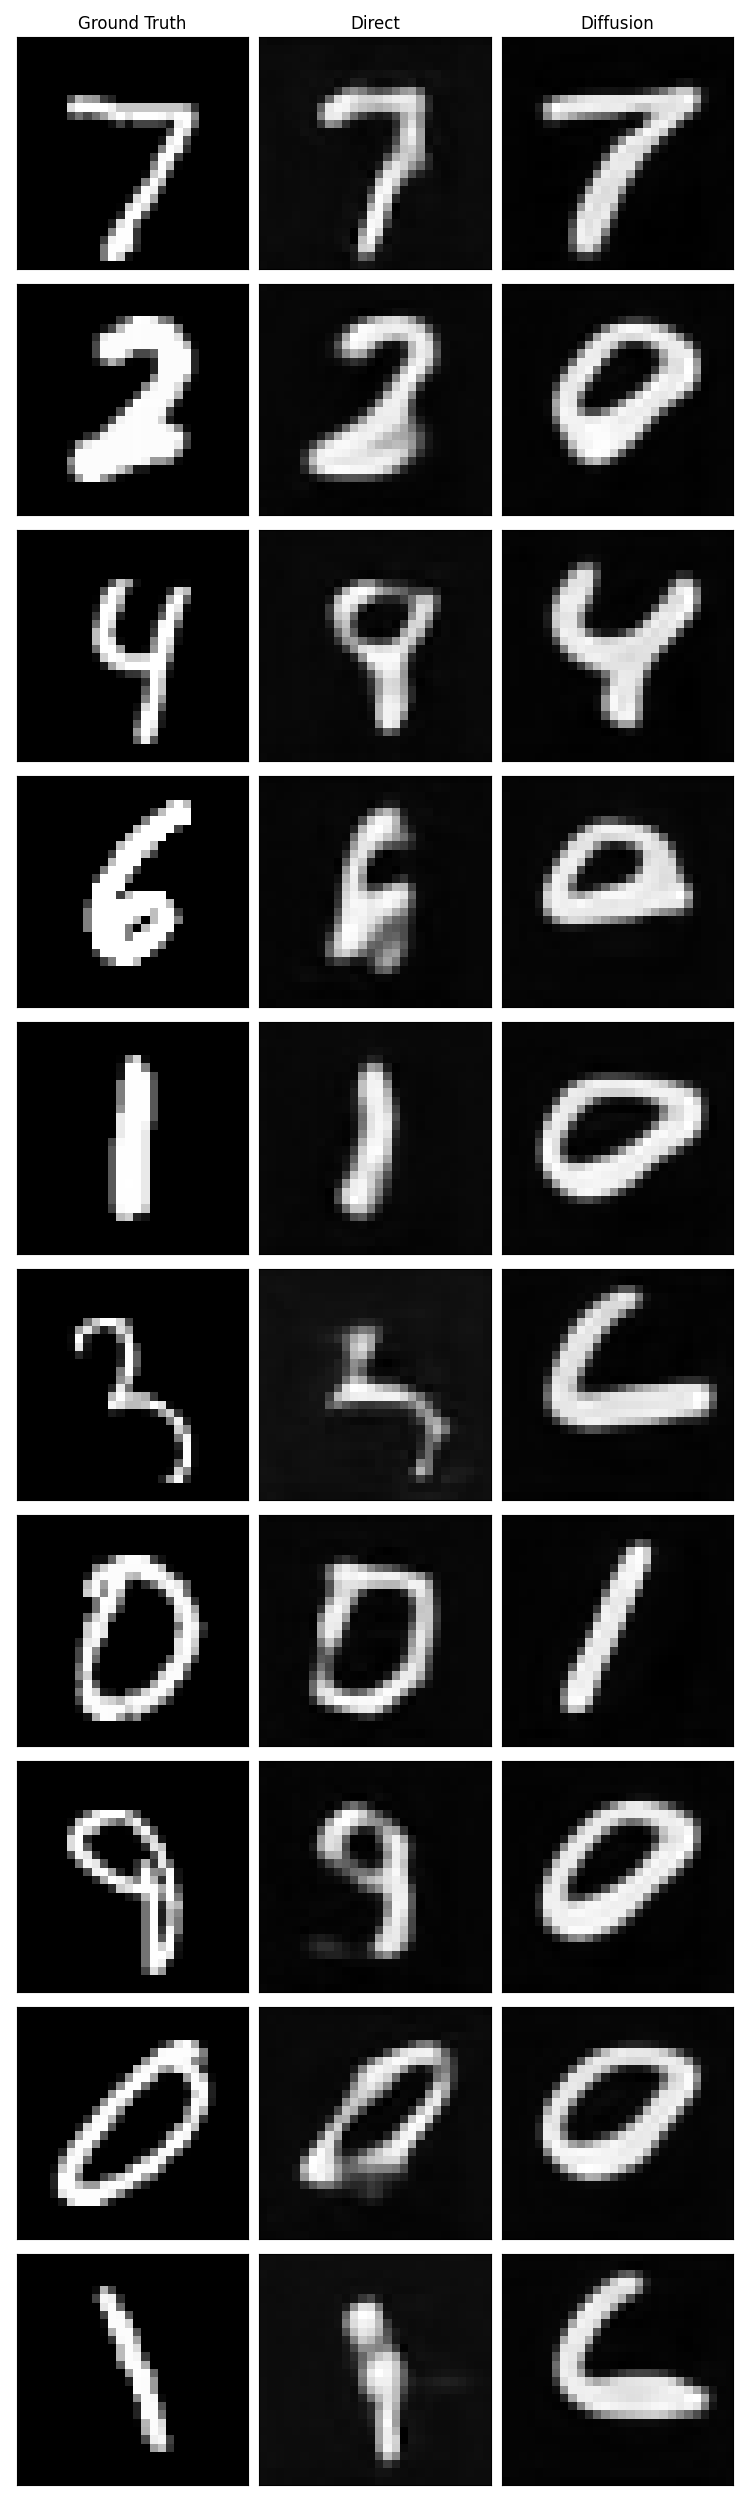
\includegraphics[width=0.9\linewidth, height=15cm, center]{figures/gt_direct_diffusion_9.png}
    \caption{First custom model}
    \label{fig:gt_direct_9}
    \end{subfigure}
    \begin{subfigure}{0.49\textwidth}
    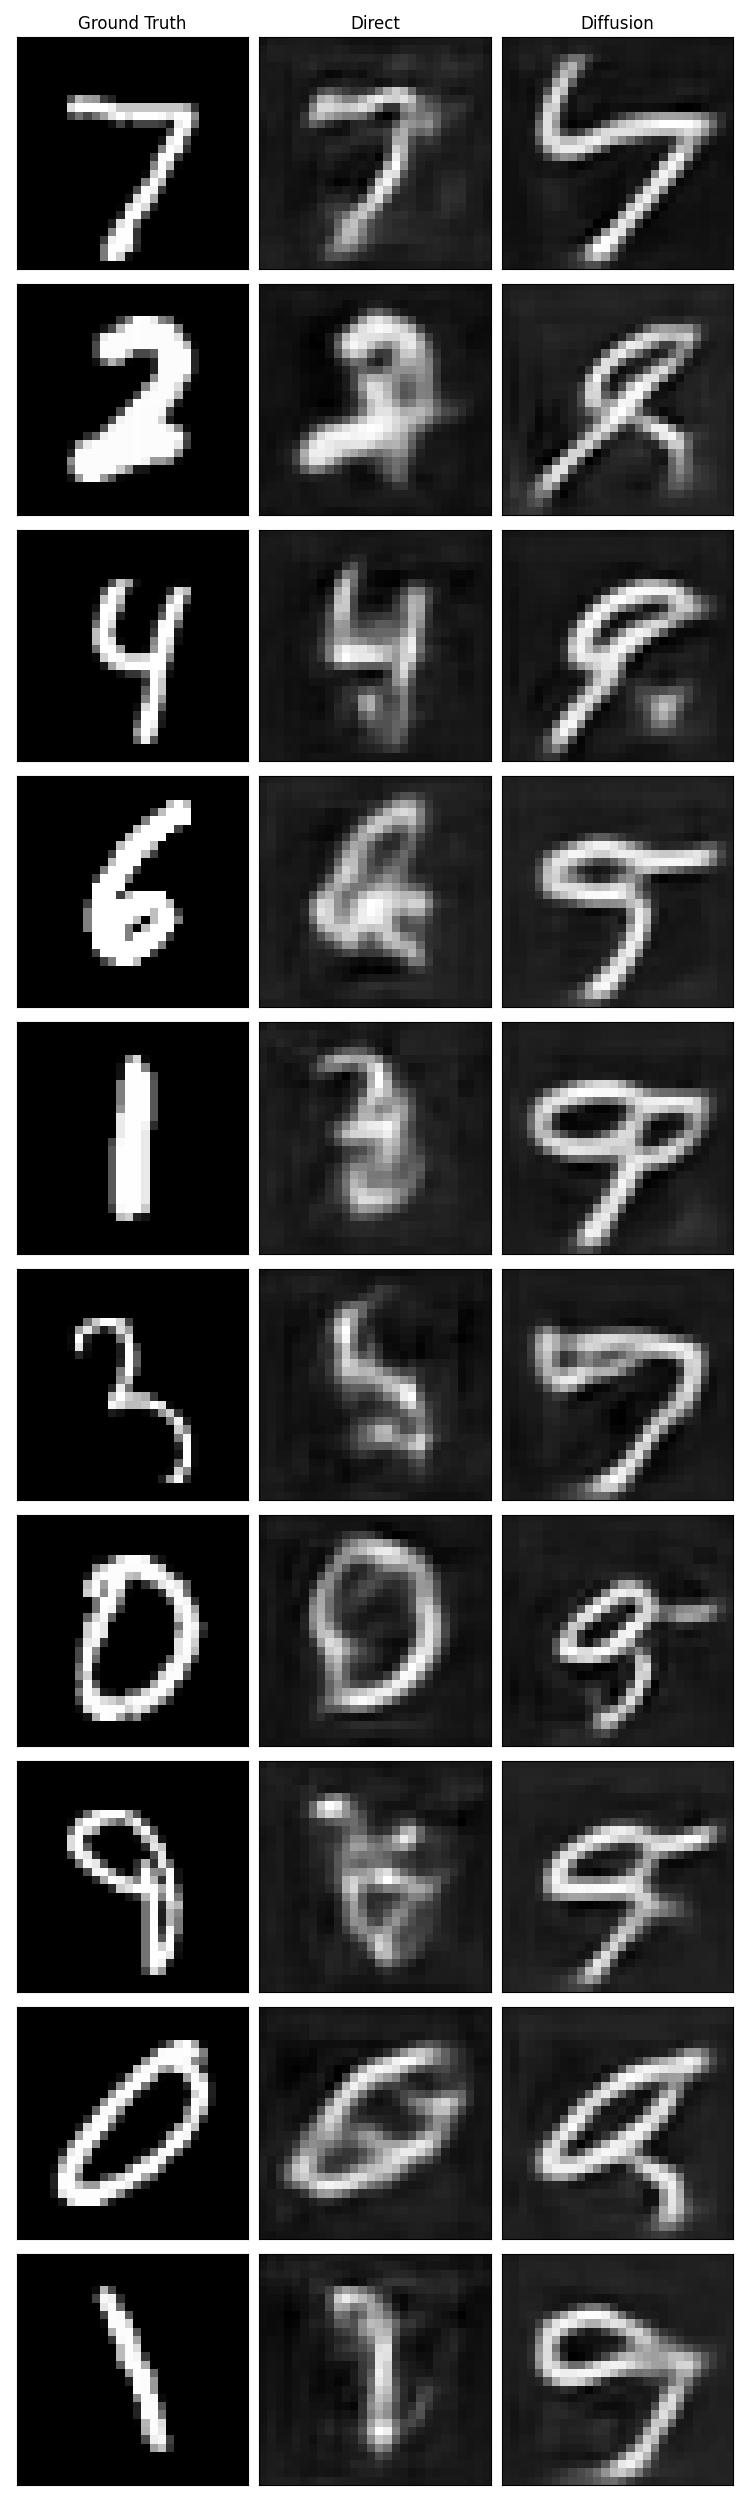
\includegraphics[width=0.9\linewidth, height=15cm, center]{figures/gt_direct_diffusion_10.png}
    \caption{Second custom model}
    \label{fig:gt_direct_10}
    \end{subfigure}

    \caption{Comparison of ground truth image vs. direct vs. diffusion generation for custom models.}
    \label{fig:cond_generation}
\end{figure}


\begin{table}[hp]
    \centering
    \begin{tabular}{| c || c | c || c | c |}
        \hline
         & \multicolumn{2}{|c||}{First model} & \multicolumn{2}{|c|}{Second model} \\
        \hline
        Digit & Direct & Diffusion & Direct & Diffusion \\
        \hline
        0 & 0.21989 & 0.38817 & 0.2735 & 0.36438 \\
        \hline
        1 & \textbf{0.15915} & \textbf{0.35128} & \textbf{0.18975} & \textbf{0.33337} \\
        \hline
        2 & 0.21640 & 0.37007 & 0.25107 & 0.34349 \\
        \hline
        3 & 0.21909 & 0.38387 & 0.23754 & 0.36732 \\
        \hline
        4 & \textbf{0.19249} & \textbf{0.36590} & \textbf{0.22798} & \textbf{0.3294} \\
        \hline
        5 & 0.20621 & 0.39696 & 0.26052 & 0.34466 \\
        \hline
        6 & 0.21506 & 0.36466 & 0.24184 & 0.35017 \\
        \hline
        7 & \textbf{0.19059} & \textbf{0.36773} & 0.24167 & \textbf{0.34073} \\
        \hline
        8 & 0.22683 & 0.37242 & 0.24823 & 0.3481 \\
        \hline
        9 & 0.19948 & 0.37203 & \textbf{0.23215} & 0.34374 \\
        \hline
        All & 0.20004 & 0.37169 & 0.23684 & 0.34449 \\
        \hline

    \end{tabular}
    \caption{Mean squared error of direct and diffusion reconstructed images, compared to ground truth. The lowest three across the labels are highlighted for each generation method.}
    \label{tab:mse_reconstruction}
\end{table}

This process was repeated for all of the sampled images with the results documented in table \ref{tab:mse_reconstruction}.
Interestingly, both models consistently appear to have the best MSE scores for 1s, 4s and 7s.
However, the actual samples produced by the second model in Figure \ref{fig:samples_10} appear to mostly resemble 8s, 9s and 5s.

\begin{figure}[hp]
    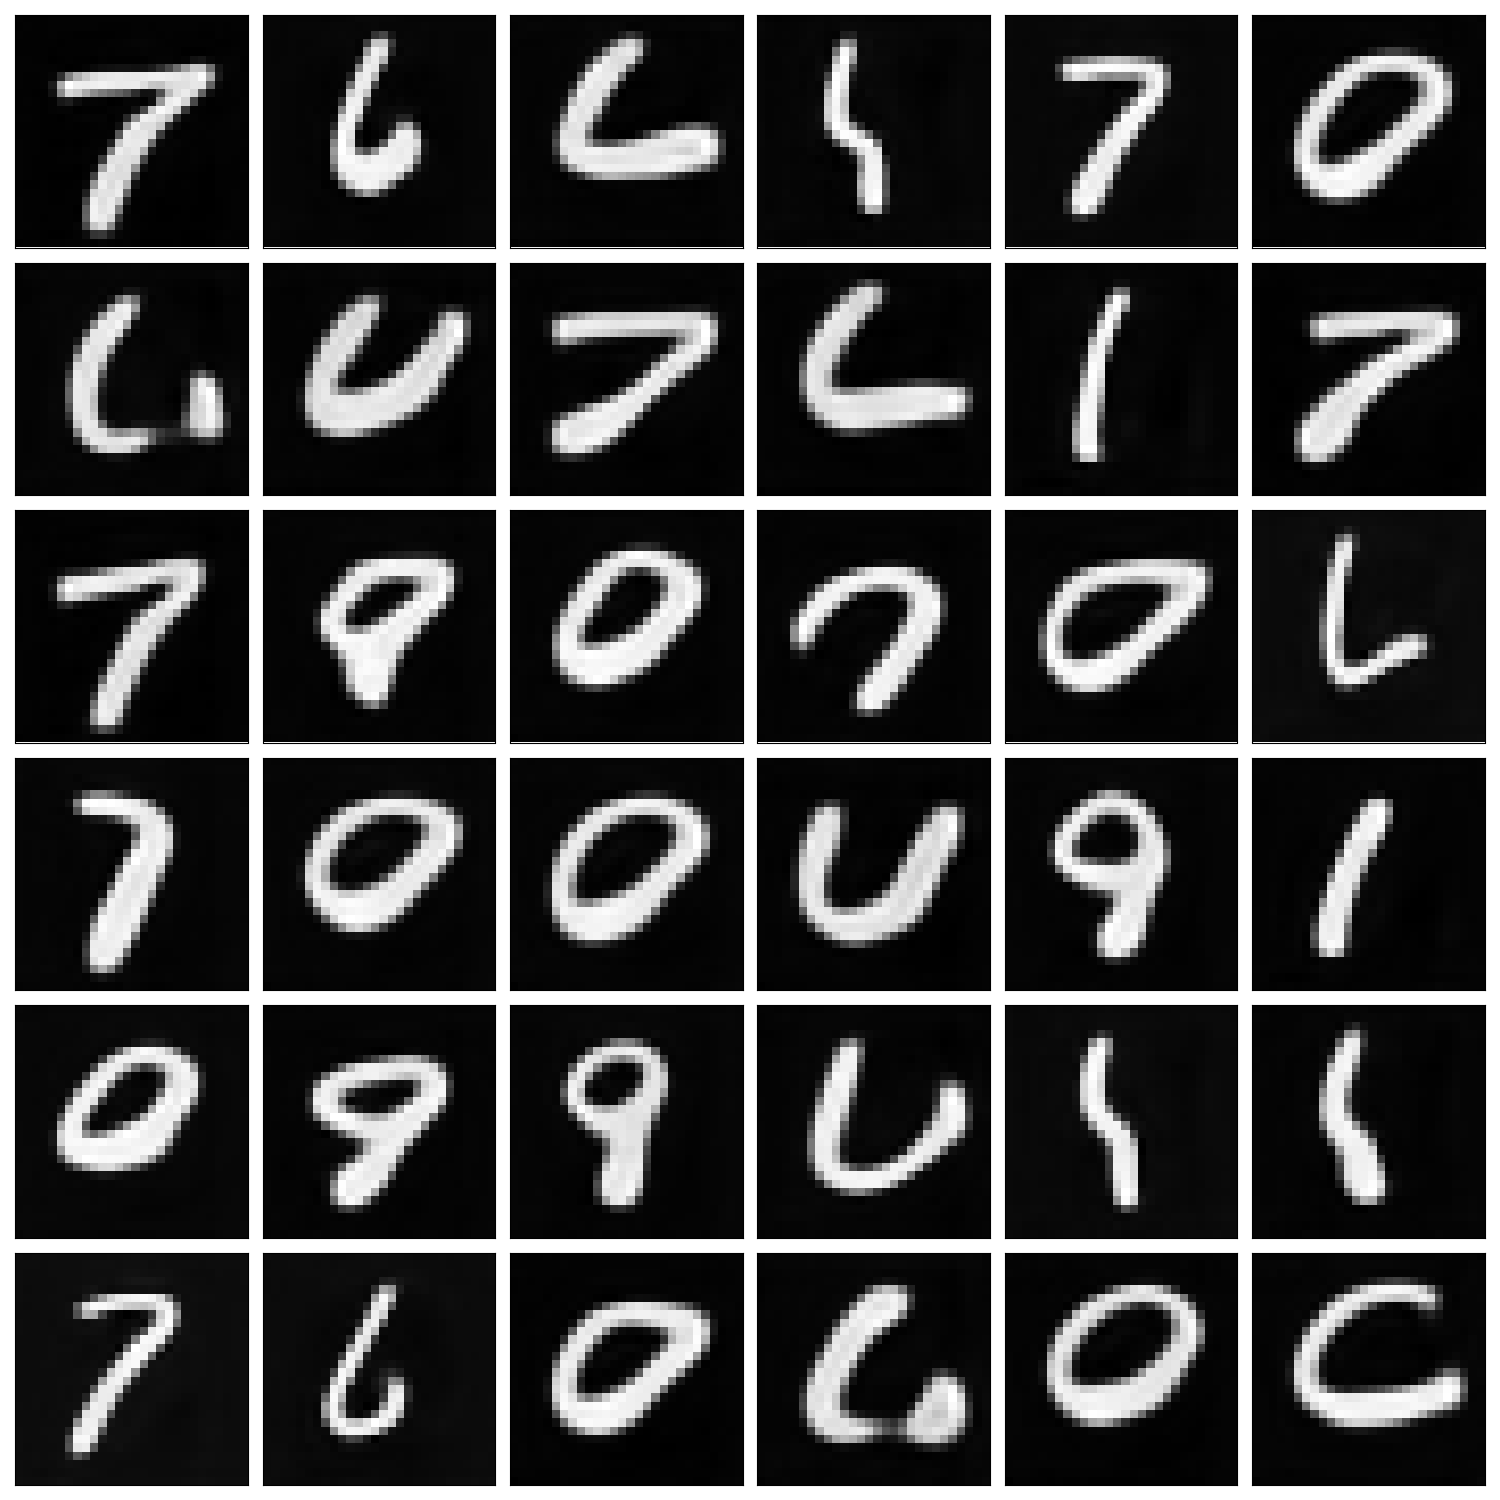
\includegraphics[scale=0.2, center]{figures/samples_9.png}
    \caption{Samples from the first final custom model.}
    \label{fig:samples_9}
\end{figure}

\begin{figure}[hp]
    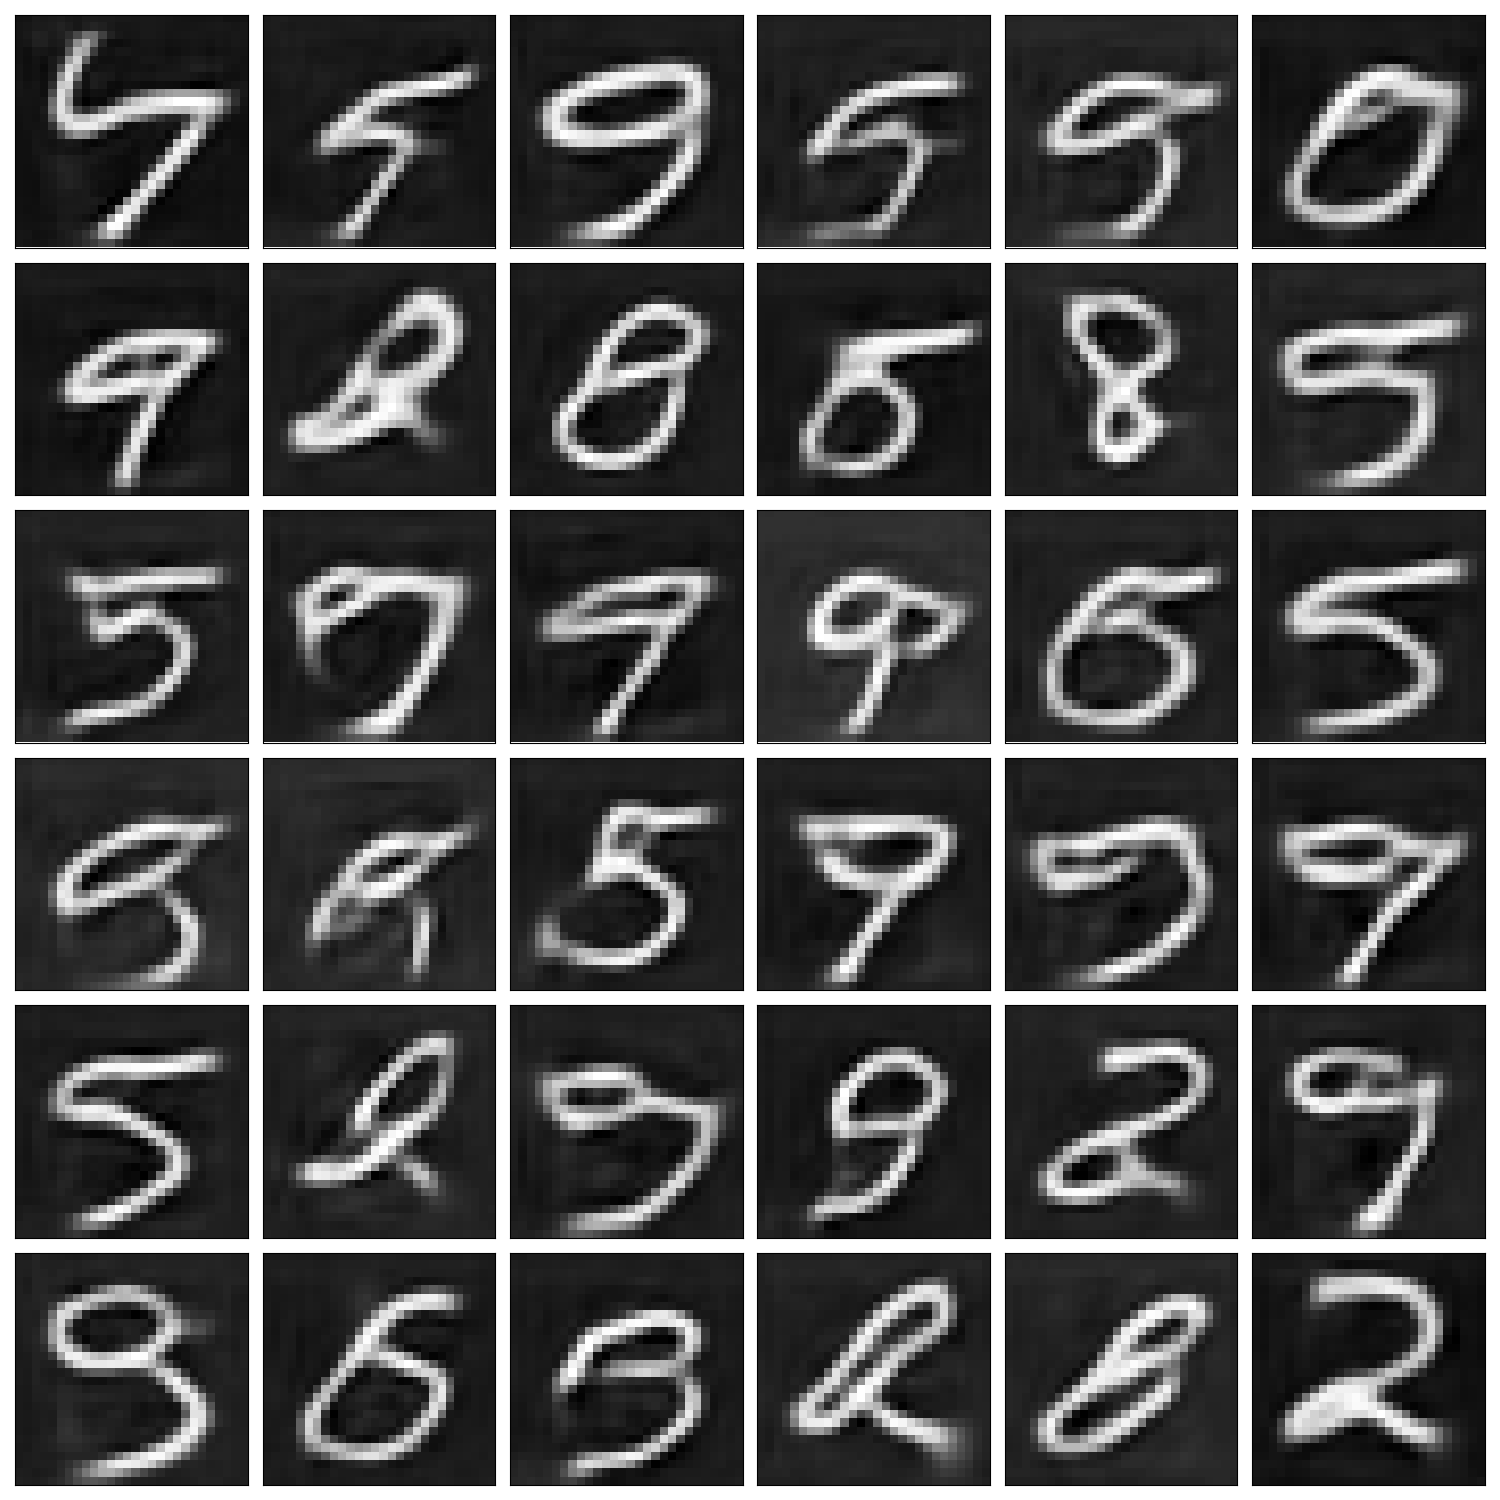
\includegraphics[scale=0.2, center]{figures/samples_10.png}
    \caption{Samples from the second final custom model.}
    \label{fig:samples_10}
\end{figure}

\subsection{Comparison of Gaussian and Custom Degradation}

As with the Gaussian degradation scheme, the samples from the custom models were transformed into t-SNE embeddings and had a Gaussian mixture model fitted,
so that an estimate of the KL divergence from the ground truth distribution could be computed.
This was much higher than the Gaussian scheme for both models, at 5.6162 for the first model, and 3.5649 for the second.
This may suggest that the original Gaussian diffusion models are much better at producing a range of images whose distribution imitates that of the ground truth data.
This is certainly evidenced by the stark comparison of Figures \ref{fig:tsne_gaussian} and \ref{fig:tsne_custom}.
In the former, the samples of images appear to cover the full ground truth embedding space more evenly, and appear in areas of high density more frequently.

However, this quantitative analysis does not necessarily correspond to the qualitative success of the two generative approaches.
Indeed, far more of the samples produced by the custom models in Figure \ref{fig:samples_9} and \ref{fig:samples_10} appear to be discernible as handwritten digits,
as compared to the Gaussian diffusion samples in Figures \ref{fig:samples_1} and \ref{fig:samples_2}.
On the other hand, the custom models appear to achieve this greater quality of generation by sacrificing sample diversity.
There is a noticeable homogeneity in the samples shows in Figures \ref{fig:samples_9} and \ref{fig:samples_10},
not just in the apparent digit class, but also in the `style' of the images.
For instance, the more realistic images produced in the second instance all seem to have the same characteristic long, thin strokes --
informally they all appear to have been produced by the same person, which is far from the case for the MNIST data.

This project highlights the challenges of evaluating generative AI models.
Attempts to quantify the performance of such models are often at odds with the judgement of a human evaluator.
Indeed, this appears to stem from the fact that their desired qualities are often at odds with eachother.
For instance, generating samples which lie close to the true underlying manifold of the ground truth data --
a quality which in itself can be challenging to quantify --
is in direct opposition to the goal of producing images that are new, rather than `learned copies' of ground truth samples.
Similarly, purely trying to optimise the model for one particular loss function can lead it to find a sub-optimal local minimum where only one ground truth class is generated,
which may explain the lack of diversity in the first custom model.

This project could be extended with further experimentation with different hyperparameter configurations, as this has been shown to be crucial in overcoming these obstacles in producing high quality generative models \cite{fi15080260}.
For instance, the underlying reconstruction model architecture could be altered, an aspect that was not considered in this project.
Additionally a subtle factor to be investigated further is the schedule of the noise parameter as a function of time.
Research suggests that this aspect of the development of diffusion models is crucial to achieving high quality synthetic images,
and that the approach should be matched to the nature of the images being generated \cite{chen2023importance}.

\bibliographystyle{IEEEtran}
\bibliography{Biblio}

\appendix

\section{Statement on the use of auto-generation tools}

Auto-generation tools, such as GitHub or Microsoft Copilot, were not used at any stage during the development of the code within the repository of this project.
Similarly, none of the content of this report was produced -- or proofread -- by modern Large Language Models such as ChatGPT at any point.

\section {High-Performance Computing Resources}

This work was performed using resources provided by the Cambridge Service for Data Driven Discovery (CSD3) operated by the University of Cambridge Research Computing Service (www.csd3.cam.ac.uk),
provided by Dell EMC and Intel using Tier-2 funding from the Engineering and Physical Sciences Research Council (capital grant EP/T022159/1),
and DiRAC funding from the Science and Technology Facilities Council (www.dirac.ac.uk).

\end{document}
